% ============================================================
%  第三卷 第十一章 双原子分子（§78–§90 + 习题）
%  底本：高教社中文版第6版（严肃 译，喀兴林 校）；OCR 错误已修正，
%  脚注已全部转录（见下方"脚注转录"块，正文不再保留圈码）
%
%  已修正的 OCR / 原书错误（对照原书页面 PNG p-291…p-338 逐条核实）：
%   1. §78：OCR"基项为 2,3,3,…"乱码按原书 p279 为 O2 基项 ^3Σ_g^-；
%      "偶态(记作^{g)})"→"偶态（记作 g）"；Σ^+／Σ^- 上标丢失补齐；
%      行11507 圈码①后补句点（原书 p291"简并①."）；
%   2. §78 习题：E_∥→E_1、E_z→E_2、U_r→U_1（§79 同）；行11563 句首
%      孤立"E_2"为 OCR 噪声，删；分离参量为斜体 A（区别于 Λ）；
%   3. §80："次数"表与 (80.1) 按原书 p283 重建（OCR 全毁）；
%      N_u,N_g 与 N_g^±,N_u^± 各式按原书 p285 修正（OCR 作 N_*,N_ε,N_B）；
%      (−1)^L P 式中指数 OCR 误作 2、t，按原书为 L；
%   4. §80 习题：谱项清单（H2,N2,Cl2,O2,HCl,CO）按原书 p286 重建，
%      OCR 下标 ε,a,e 均为 g,u 之误；"处 $\bar{\pmb{\mathscr{F}}}^2$"→"处于"；
%   5. §81：H2 基项 OCR"15 谱项"→^1Σ 谱项；"x+1"→"对^1Σ谱项"；
%      Cs^*→Cs^+、F→F^-；SO2,SO3,HClO2…中 0→O；行11789"铜族"→"锕族"；
%      3d→4p 跃迁（OCR 作 4_P）；
%   6. §81 习题：(2) e^{-π}→e^{-r_1}；(4)(5) 的 U_κ,U_μ→U_g,U_u；
%      参考文献乱码按原书 p290 为（Л. Д. Ландау,1961; C. Herring,1961）；
%   7. §82：(82.14) B_r→B_v；(82.12) ΔE_ν→ΔE_v；U_★,B_★,ω_★→U_e,B_e,ω_e；
%      K_z（OCR 作 K_s）；习题"K和量子数"→"K 和 v 量子数"（p296）；
%   8. §83："轨道自动量"系原书 p298 排印之误，改"轨道角动量"；
%      行12099"与∑2成正比"→"与Σ^2 成正比"、句内多余"∑^2"删；
%      "所差的AA"→"所差的 AΛ"；
%   9. §84：行12178"n̄=常数×K̂"依原书 p300 重建（OCR 乱码）；
%      题2 久期方程依原书 p303 重建（OCR 全毁）；题1 α_*→α_e；
%      题3 ⟨J|n·S|J∓1⟩ 两式按原书 p303；
%  10. §85：Λ_𝒳→Λ_实（"分子实"之实）；0^+/0^- 谱项符号补齐；
%      N_g=N_u+1 等四式下标按原书 p305 修正；
%  11. §86：(86.2) 左端 g_s/g_s→g_s/g_a；Σ_g^+,Σ_u^+,Σ_g^-,Σ_u^- 各处
%      按原书 p308 修正（OCR 之 ∑_β,∑_μ,∑_κ 均为 g,u 之误）；
%  12. §87：(87.2) 补 OCR 丢失的第二式 ⟨n′,K−1,Λ∥A∥nKA⟩=i√((K²−Λ²)/K)…；
%      (87.4) 第二式 K²−1→K²−Λ²（据 Λ=0 特例反推并核 p310 原书）；
%      情形a 式按原书 p310 为 ⟨n′ΩΛ|A_ζ|nΩΛ⟩（OCR 重复"n,"）；
%      情形b 末式 A_ξ→A_ζ；习题1 分子 Q→Ω（原书排印之误，p311）；
%  13. §88：(88.2)—(88.5) 中"常数"二字 OCR 乱码按原书 p313 重建；
%      (88.4)"常数−A²/ε"→"常数∼A²/ε"；R. Kronlg→R. Kronig（原书排印之误）；
%  14. §89：(89.2)—(89.4) 分子"常数"按原书 p315 重建；习题 E_0（OCR 作 F_0）；
%      行12653"近距离"按物理与原书 p316 改"远距离"（原书排印之误）；
%  15. §90：(90.3) χ_N→χ_{N1}；行12794"χ_N=rψ_N(ψ_N为…)"句读按原书；
%      行12786 处分式 dp₁/dr₀−dp₂/dr₀ 系原书排印（导数在 r₀ 取值），照排；
%      题3 艾里函数公式按原书 p325 重建（F_{J1},F_{J2}）；
%      题4 О. Б. Фирсов（OCR 乱码）；题4 末式中间步 ρ^3/2→ρ^2、e^{-p}→e^{-ρ}
%      （按 ∫₀^∞ e^{-ρx}dx/√x=√(π/ρ) 核算，与原书最终答案一致）；
%  16. 其它：函数名正体（\cos,\sin,\exp）、\mathrm{e}、\mathrm{d} 收紧；
%      俄文人名复原（Л. Д. Ландау 等）；全角标点按文体约定。
%
%  遗留问题（OCR 存疑，已照原书页面排版）：
%   - §88 行12561 原书印作"根据(88.1)′式"，撇号疑为排印残留，照原书保留；
%   - §81 习题解 (1) 式积分号右端因子按原书 p291 照排（未作量纲复核）；
%   - §90 题2 分母原书印作"|F_2^{-}F_1|"（上标减号），按 |F_2-F_1| 排；
%   - （已解决）原圈码脚注文本已全部补录，见下方"脚注转录"块。
%
%  脚注转录（脚注代理，2026-10-11，按 pages300 p291–p338 页面实况逐条核录，
%  共 47 处：\footnote 取代原圈码，footmisc[perpage] 按页自动圈码）：
%   - 页码分布：p291(1) p292(2) p295(1) p298(2) p300(2) p301(1) p302(1)
%     p303(2) p304(2) p305(1) p306(1) p307(1) p308(1) p309(1) p310(2)
%     p311(2) p312(1) p313(1) p316(1) p318(2) p319(4) p320(2) p321(1)
%     p324(1) p327(2) p328(2) p329(2) p330(1) p331(2) p335(1) p338(1)；
%   - 公式类脚注：p304②（$U_g-U_u=-1.64R^{5/2}\mathrm{e}^{-2R}$）、
%     p307①（$\psi_{\mathrm{rot}}$ 显示式，footnote 内 equation*）、
%     p308①（$U_e,\hbar\omega_e,B_e$ 数值表，tabular 排入脚注）、
%     p309①（质心动能式）、p316①（$E^{(0)}$ 式）；
%   - p328 脚注②原书印"等与 6.5"系排印误，按上下文改"等于 6.5"；
%   - p309 脚注①质心动能式第二处印作 $\boldsymbol{P}_{\parallel}/2(M_1+M_2)$
%     （俄文原本作 $P^2/2(M_1+M_2)$），照原书页面照排并在此备案；
%   - 行11507"重简并①"原书 p291 页脚（脚注页码对照表无该锚点，以页面为准）；
%     p307/p316/p321/p324 诸锚点同按页面实况定位。
% ============================================================
\chapter{双原子分子}

\section{双原子分子的电子谱项}

在分子理论中，原子核质量远大于电子质量这一事实起着重要的作用.由于这种质量差别，分子中原子核的运动速度远小于电子速度.这就有可能把电子的运动看作是电子在相隔一定距离的一些固定原子核之间的运动.对这样一种系统求出的能级 $U_n$，就称为分子的电子谱项.电子谱项与原子能级（它是一组数值）不同，它不是一组数值而是以分子中各个原子核间距离为参量的一个函数.$U_n$ 中还包含原子核之间相互作用的静电能量，所以 $U_n$ 实质上就是当诸固定的原子核具有给定排列时的分子总能量.

我们先从类型最简单的分子——双原子分子考虑起，它可以供我们进行最完备的理论研究.双原子分子的电子谱项只是核距 $r$ 这一个参量的函数.

原子谱项是按总轨道角动量 $L$ 的数值加以分类的，这是原子谱项分类工作中的一个首要原则.但在分子中并不存在电子总轨道角动量的守恒律，因为多个原子核的电场并不是一个有心力场.

可是在双原子分子中，电场对两个原子核的连线而言具有轴对称性.由于轨道角动量沿该轴的分量是一个守恒量，我们可按该分量的各种数值对分子的电子谱项进行分类.沿分子轴的总轨道角动量分量，其绝对值习惯上记作 $\Lambda$；$\Lambda$ 的取值 $0,1,2,\cdots$，$\Lambda$ 值不同的各个谱项通常用大写的希腊字母加以区别，这些希腊字母与 $L$ 值不同的原子谱项所用的各个拉丁字母相对应.例如 $\Lambda=0,1,2$ 时分别称为 $\Sigma$，$\Pi$ 和 $\Delta$ 谱项.较大的 $\Lambda$ 值通常可不考虑.

其次，分子的每个电子态是由该分子中所有电子的总自旋 $S$ 加以标志的.如果 $S$ 不等于零，对总自旋的空间方向而言就有 $2S+1$ 重简并\footnote{在这里我们略去了来自相对论作用的精细结构（见后面 §83 和 §84）.}和原子的情形一样，数值 $2S+1$ 称为该谱项的多重度，并把它标记在该谱项字母的左上角，例如 $^3\Pi$ 代表 $\Lambda=1$，$S=1$ 的谱项.

分子的对称性除了能绕对称轴旋转任意角度以外，还可以对通过对称轴的任一平面进行反射，如果我们施行这样的一次反射，分子的能量保持不变.可是，反射以后所得的态并不完全等同于原来的态.因为，对通过分子轴的一个平面进行一次反射后，沿该轴的角动量（它是一个轴矢量）要变号.于是我们得出结论，$\Lambda$ 值不等于零的所有电子谱项都是双重简并的：每个能量值对应两个态，这两个态中轨道角动量沿分子轴的投影方向是相反的.在 $\Lambda=0$ 的情形中，分子态对反射完全不变，因此 $\Sigma$ 谱项并不简并，反射的结果 $\Sigma$ 谱项的波函数只是改变了一个常数倍.由于对同一平面的两次反射等于一个恒等变换，这个常数只能是 $\pm1$.因此我们有必要把波函数反射后保持不变的 $\Sigma$ 谱项与波函数反射后变号的 $\Sigma$ 谱项区分开来.前者记作 $\Sigma^+$，后者记作 $\Sigma^-$.

如果分子是由两个相同原子组成的，就会出现一种新的对称性，使它的电子谱项多出一个标记.原子核全同的一个双原子分子，在原子核联线的中点处具有一个对称中心\footnote{还有一个对称面，即分子轴的垂直平分面.但是这个对称元素无需单独考虑，有了对称中心和对称轴后就能自动给出这个对称面.}（我们把它取作原点）.因而哈密顿量对分子中所有电子坐标的同时变号（原子核坐标不变号）保持不变.由于上述变换算符\footnote{不要和分子中所有粒子坐标的同时反演混淆起来（参考 §86）.}也和总轨道角动量算符相对易，我们就有可能把具有给定 $\Lambda$ 值的谱项按其宇称分类：电子坐标变号时，偶态（记作 $g$）的波函数保持不变，奇态（记作 $u$）的波函数改变符号，代表宇称的下标 $u$ 和 $g$ 按惯例放在谱项字母的右下角，例如 $\Pi_u$，$\Pi_g$，等等.

下面是一个经验事实，绝大多数具有化学稳定性的双原子分子的电子基态是完全对称的：电子波函数对分子的所有对称变换一律保持不变.绝大多数情形下基态的总自旋 $S$ 还等于零.换句话说，分子的基项为 $^1\Sigma^+$，如果该分子由两个相同原子所组成，则为 $^1\Sigma_g^+$.这些规则的例外有 $\mathrm{O}_2$ 分子（基项为 $^3\Sigma_g^-$）和 NO 分子（基项为 $^2\Pi$）.

\begin{xiti}

对于 $\mathrm{H}_2^+$ 离子的电子谱项的薛定谔方程，试用椭圆坐标分离其变量.

解：在两个静止质子的电场中，单电子的薛定谔方程为（采用原子单位）
\begin{equation*}
  \nabla^2\psi+2\left(E+\frac{1}{r_1}+\frac{1}{r_2}\right)\psi=0,
\end{equation*}
椭圆坐标 $\xi$，$\eta$ 由下式定义：
\begin{equation*}
  \xi=\frac{r_1+r_2}{R},\qquad\eta=\frac{r_2-r_1}{R};\qquad
  1\leqslant\xi\leqslant\infty,\ -1\leqslant\eta\leqslant1.
\end{equation*}
第三个坐标 $\varphi$ 就是绕两核连线的转角，$R$ 是两核的间距（见《力学》，§48）.这个坐标系中的拉普拉斯算符为
\begin{equation*}
  \nabla^2=\frac{4}{R^2(\xi^2-\eta^2)}
  \left[\frac{\partial}{\partial\xi}(\xi^2-1)\frac{\partial}{\partial\xi}
  +\frac{\partial}{\partial\eta}(1-\eta^2)\frac{\partial}{\partial\eta}\right]
  +\frac{1}{R^2(\xi^2-1)(1-\eta^2)}\frac{\partial^2}{\partial\varphi^2}.
\end{equation*}
令
\begin{equation*}
  \psi=X(\xi)Y(\eta)\mathrm{e}^{\mathrm{i}\Lambda\varphi},
\end{equation*}
我们得下列 $X$ 和 $Y$ 的方程
\begin{equation*}
  \frac{\mathrm{d}}{\mathrm{d}\xi}\left[(\xi^2-1)\frac{\mathrm{d}X}{\mathrm{d}\xi}\right]
  +\left(\frac{1}{2}ER\xi^2+2R\xi+A-\frac{\Lambda^2}{\xi^2-1}\right)X=0,
\end{equation*}
\begin{equation*}
  \frac{\mathrm{d}}{\mathrm{d}\eta}\left[(1-\eta^2)\frac{\mathrm{d}Y}{\mathrm{d}\eta}\right]
  +\left(-\frac{1}{2}ER\eta^2-A-\frac{\Lambda^2}{1-\eta^2}\right)Y=0,
\end{equation*}
式中 $A$ 是分离参量.

每个电子谱项 $E(R)$ 由三个量子数描述：$\Lambda$ 以及两个“椭圆量子数”$n_\xi$ 和 $n_\eta$，后者确定了函数 $X(\xi)$ 和 $Y(\eta)$ 的零点数目.

\end{xiti}

\section{电子谱项的相交}

双原子分子中的电子谱项作为核距 $r$ 的函数可以用能量对 $r$ 的作图法表出，考察代表不同谱项的不同曲线的相交问题颇有意义.

设 $U_1(r)$ 和 $U_2(r)$ 是两个不同的电子谱项.如果它们相交于某一点，那么函数 $U_1$ 和 $U_2$ 在该点附近就会有接近值.为了判断怎样才能相交，最好对问题进行以下的处理.我们考虑一个 $r_0$ 点，该点处的 $U_1(r)$ 和 $U_2(r)$ 函数值十分接近（我们记作 $E_1$ 和 $E_2$）但是并不相等，现在来看一下该点位移一个很短的距离 $\delta r$ 后能不能使 $U_1$ 和 $U_2$ 值变得相等.能量 $E_1$ 和 $E_2$ 是核距为 $r_0$ 的场内多电子系统哈密顿量 $\hat{H}_0$ 的两个本征值.如果使距离 $r_0$ 增加 $\delta r$，哈密顿量变成 $\hat{H}_0+\hat{V}$，其中的 $\hat{V}=\delta r\cdot\partial\hat{H}_0/\partial r$ 是一个小的改正，函数 $U_1$ 和 $U_2$ 在 $r_0+\delta r$ 点的值可看作这个新哈密顿量的本征值.这个观点使我们可以用微扰论求出 $U_1(r)$ 和 $U_2(r)$ 谱项在 $r_0+\delta r$ 点的值，$\hat{V}$ 看成算符 $\hat{H}_0$ 的一个微扰.

可是，通常的微扰论方法在这里并不适用，因为未微扰问题中的能量本征值 $E_1$ 和 $E_2$ 十分接近，其差值一般讲来并不远大于微扰量，条件(38.9)式并不满足.由于差值 $E_2-E_1$ 趋于零时变成有简并的本征值情形，我们自然可试用类似于§39中的方法去解决具有相近本征值的问题.

设 $\psi_1,\psi_2$ 是未微扰算符 $\hat{H}_0$ 的两个本征函数，属于能量 $E_1,E_2$.我们不用 $\psi_1$ 和 $\psi_2$ 而用下列线性组合作为零级近似
\begin{equation}
  \psi=c_1\psi_1+c_2\psi_2.
\end{equation}
把上式代入受微扰方程
\begin{equation}
  (\hat{H}_0+\hat{V})\psi=E\psi
\end{equation}
得到
\begin{equation*}
  c_1(E_1+\hat{V}-E)\psi_1+c_2(E_2+\hat{V}-E)\psi_2=0,
\end{equation*}
对上式分别左乘 $\psi_1^*$ 和 $\psi_2^*$，积分后得到两个代数方程
\begin{equation}
\left.\begin{aligned}
  &c_1(E_1+V_{11}-E)+c_2V_{12}=0,\\
  &c_1V_{21}+c_2(E_2+V_{22}-E)=0,
\end{aligned}\right\}
\end{equation}
由于算符 $\hat{V}$ 是自轭的，矩阵元 $V_{11}$ 和 $V_{22}$ 是实数并且 $V_{12}=V_{21}^*$.以上两式的相容条件为
\begin{equation*}
  \left|\begin{array}{cc}
    E_1+V_{11}-E & V_{12}\\
    V_{21} & E_2+V_{22}-E
  \end{array}\right|=0
\end{equation*}
因而
\begin{equation}
\begin{aligned}
  E&=\frac{1}{2}(E_1+E_2+V_{11}+V_{22})\ \pm\\
  &\pm\sqrt{\frac{1}{4}(E_1-E_2+V_{11}-V_{22})^2+|V_{12}|^2}.
\end{aligned}
\end{equation}
上式给出了欲求的一级近似能量本征值.

如果在 $r_0+\delta r$ 处这两个谱项的能量值相等（即谱项相交），这就意味着(79.4)式给出的两个 $E$ 值相等.为此必须令(79.4)根号中的表式等于零.由于它是两个平方项之和，故谱项存在交点的条件是
\begin{equation}
  E_1-E_2+V_{11}-V_{22}=0,\qquad V_{12}=0.
\end{equation}
可是，可供我们支配的决定微扰 $\hat{V}$ 的只有一个任意参量，即位移量 $\delta r$.因此(79.5)的两个方程一般讲来不能同时满足（假定 $\psi_1,\psi_2$ 已选成实函数，故 $V_{12}$ 也是实的）.

但也有可能碰到 $V_{12}$ 矩阵元恒等于零的情形，此时(79.5)只留下一个方程，适当选择 $\delta r$ 可使该方程得到满足.这种情形总是发生在所考虑的两个谱项具有不同对称性的时候.这里所讲的对称性是指所有可能的对称形式：绕轴转动，对平面的反射，反演，也指电子的对换.在双原子分子中，这意味着所指的是具有不同 $\Lambda$ 值，不同宇称或不同多重度的谱项，或者是指（对 $\Sigma$ 谱项而言）$\Sigma^+$ 和 $\Sigma^-$ 谱项.

上述论断的成立，在于微扰算符（和哈密顿量本身一样）与分子的所有对称算符相对易，包括沿轴的角动量算符，反射和反演算符以及电子的对换算符.

§29和§30中曾经证明，对于一个与角动量及反演算符都对易的标量算符而言，它的非零矩阵元只有角动量和宇称都相同的状态之间的跃迁矩阵元.一般情形下，当所对易的算符为任意的对称算符时，这个证明仍能成立.我们不在这里重复这个证明，因为§97中将在群论基础上给出另一个普遍证明.

因此我们得到这样的结论，双原子分子中只有对称性不同的谱项才能相交，对称性相同的谱项是不能相交的（E.~Wigner, J.~von Neumann, 1929）.如果在某种近似计算的结果中，我们得到了对称性相同的两个相交谱项，那么在下一级的近似计算中它们就会分开，如图~27 的实线所示.

\par\nopagebreak\noindent\begin{minipage}{\linewidth}\centering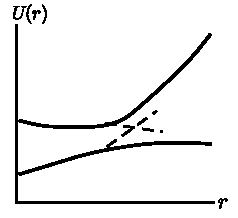
\includegraphics[width=5cm]{fig27.pdf}\\[0.3em]{\small 图 27}\end{minipage}\par\nopagebreak

应该强调的是，这个结论不只是对双原子分子成立，而且是量子力学的一个普遍定理：只要哈密顿量中含有某个参量从而它的本征值是该参量的函数时，这个结论即能成立.

采用群论的术语（见§96），谱项有可能相交的一般条件是，这两个谱项应该分属于系统哈密顿量对称群的两个不同的不可约表示\footnote{这个规则的表观例外是 $\mathrm{H}_2^+$ 离子的电子谱项.它们由角动量分量 $\Lambda$ 以及两个椭圆量子数 $n_\xi$ 和 $n_\eta$ 来描述（见 §78，例题），由于这些量子数分别与不同变量的函数相联系，这就无法阻止 $\Lambda$ 值相同而 $n_\xi$ 和 $n_\eta$ 值不同的两个 $E(R)$ 谱项相交，即使这些谱项对旋转和反射具有相同的对称性.但实际上，该系统的薛定谔方程中变量的可分离性，说明了它的哈密顿量尚有来自几何性质以外的更高对称性，相对于这个完整对称群而言，$n_\xi$ 和 $n_\eta$ 值不同的态具有不同的对称类型.}.

多原子分子中，电子谱项不是一个参量而是若干个参量的函数，这些参量就是各个核距.令 $s$ 为独立核距数.在具有 $N$ 个（$N>2$）原子的分子中，当原子核可任意排列时，这个数 $s=3N-6$.从几何学的观点看来，每个 $U_n(r_1,\cdots,r_s)$ 谱项是 $s+1$ 维空间中的一个曲面，这些曲面的交区可以有不同的维数，从0维（交于一点）到 $s-1$ 维.除了微扰 $\hat{V}$ 现在不是由一个参量而是由 $s$ 个参量 $\delta r_1,\cdots,\delta r_s$ 所确定的以外，上面所作的推导全部有效.即使是两个参量，(79.5)中的两个方程式一般讲来总能得到满足.因此得出这样的结论：多原子分子中任意两个谱项都有可能相交.如果这两个谱项具有相同的对称性，则其交区由(79.5)式的两个条件所确定，从而这个交区是 $s-2$ 维的.如果这两个谱项具有不同的对称性，(79.5)式中只留下一个条件，这个交区是 $s-1$ 维的.

例如 $s=2$ 时，谱项可表为三维坐标系中的曲面.当谱项的对称性不同时，这些曲面的交线是一条直线（$s-1=1$），而当对称性相同时，则交于一点（$s-2=0$）.在后一种情形下，不难判明交点附近的曲面形状.谱项交点附近的能量值是由(79.4)式给出的.该式中的矩阵元 $V_{11},V_{22},V_{12}$ 是位移 $\delta r_1,\delta r_2$ 的线性函数，因而也是距离 $r_1,r_2$ 本身的线性函数.由解析几何知道，这样的一个方程确定了一个椭圆锥面.因此这两个谱项在交点附近可以表成任意放置的一个双椭圆锥面（图~28）.

\par\nopagebreak\noindent\begin{minipage}{\linewidth}\centering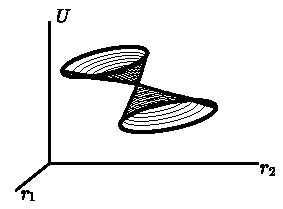
\includegraphics[width=6cm]{fig28.pdf}\\[0.3em]{\small 图 28}\end{minipage}\par\nopagebreak

\section{分子谱项与原子谱项的关系}

当我们增大双原子分子内原子核间的距离时，其极限是两个孤立原子（或离子）.因此就产生了分子的电子谱项与分开后所得的原子态之间的对应关系问题（E.~Wigner, E.~Witmer, 1928）.这种关系并不是单值的：如果把两个给定态的原子靠拢起来，所得的分子可以具有各种不同的电子态.

我们先假定该分子是由两个不同原子组成的.设孤立原子分别处于轨道角动量为 $L_1,L_2$ 自旋为 $S_1,S_2$ 的态中，并令 $L_1\geqslant L_2$.角动量沿原子核连线的投影值可取 $M_1=-L_1,-L_1+1,\cdots,L_1$ 和 $M_2=-L_2,-L_2+1,\cdots,L_2$.$M_1$ 和 $M_2$ 的绝对值确定了这两个原子靠拢后所得的 $\Lambda$ 值.把 $M_1$ 和 $M_2$ 的各种可能值相加起来，我们发现所得的各种 $\Lambda=|M_1+M_2|$ 值的次数如下：
\begin{equation*}
\begin{array}{rl}
  \Lambda=L_1+L_2 & \text{2次，}\\
  L_1+L_2-1 & \text{4次，}\\
  \cdots\cdots\cdots\cdots \\
  L_1-L_2 & \text{2(}2L_2+1\text{)次，}\\
  L_1-L_2-1 & \text{2(}2L_2+1\text{)次，}\\
  \cdots\cdots\cdots\cdots \\
  1 & \text{2(}2L_2+1\text{)次，}\\
  0 & \text{2}L_2+1\text{次，}
\end{array}
\end{equation*}
我们记得，$\Lambda\neq0$ 的谱项都是双重简并的，$\Lambda=0$ 的谱项都是无简并的，因此有：
\begin{equation}
\left.\begin{aligned}
  &\Lambda=L_1+L_2\ \text{的谱项共}\ 1\ \text{个，}\\
  &\Lambda=L_1+L_2-1\ \text{的谱项共}\ 2\ \text{个，}\\
  &\qquad\cdots\cdots\cdots\cdots\\
  &\Lambda=L_1-L_2\ \text{的谱项共}\ 2L_2+1\ \text{个，}\\
  &\Lambda=L_1-L_2-1\ \text{的谱项共}\ 2L_2+1\ \text{个，}\\
  &\qquad\cdots\cdots\cdots\cdots\cdots\cdots\cdots\cdots\\
  &\Lambda=0\ \text{的谱项共}\ 2L_2+1\ \text{个；}
\end{aligned}\right\}
\end{equation}
一共有 $(2L_2+1)(2L_1+1)$ 个谱项，它们的 $\Lambda$ 值从0到 $L_1+L_2$.

两个原子的自旋 $S_1,S_2$ 按角动量相加的一般规则组合成为分子的总自旋，给出下列各个可能的 $S$ 值：
\begin{equation}
  S=S_1+S_2,\ S_1+S_2-1,\ \cdots,\ |S_1-S_2|.
\end{equation}
把每个 $S$ 值和(80.1)中的各个 $\Lambda$ 值组合起来，即得所合成的分子中所有可能谱项的完整的清单.

对于 $\Sigma$ 谱项，还有一个符号问题.这个问题是很易解决的，只需注意到当 $r\to\infty$ 时，分子波函数可以表成两个原子波函数的乘积（或乘积之和）.$\Lambda=0$ 的角动量既可以从不等于零但有 $M_1=-M_2$ 的两个原子角动量相加而成，也可以从 $M_1=M_2=0$ 的两个原子角动量相加而成.我们用 $\psi_{M_1}^{(1)}$，$\psi_{M_2}^{(2)}$ 代表第一个和第二个原子的波函数.当 $M=|M_1|=|M_2|\neq0$ 时，可作以下的对称乘积和反对称乘积：
\begin{equation*}
\begin{aligned}
  \psi^+&=\psi_M^{(1)}\psi_{-M}^{(2)}+\psi_{-M}^{(1)}\psi_M^{(2)},\\
  \psi^-&=\psi_M^{(1)}\psi_{-M}^{(2)}-\psi_{-M}^{(1)}\psi_M^{(2)}.
\end{aligned}
\end{equation*}
对竖直平面（即通过分子轴的一个平面）的反射使角动量的轴向投影变号，从而使 $\psi_M^{(1)}$，$\psi_M^{(2)}$ 分别变成 $\psi_{-M}^{(1)}$，$\psi_{-M}^{(2)}$，以及反之.此时函数 $\psi^+$ 保持不变而 $\psi^-$ 变一符号，前者对应于 $\Sigma^+$ 谱项，后者对应于 $\Sigma^-$ 谱项.因此对于每个 $M$ 值，得到一个 $\Sigma^+$ 谱项和一个 $\Sigma^-$ 谱项.由于 $M$ 可以取 $L_2$ 个不同的值（$M=1,\cdots,L_2$），总共有 $L_2$ 个 $\Sigma^+$ 谱项和 $L_2$ 个 $\Sigma^-$ 谱项.

另一方面，若 $M_1=M_2=0$，分子波函数的形式为 $\psi=\psi_0^{(1)}\psi_0^{(2)}$.为了判明 $\psi_0^{(1)}$ 函数对竖直平面的反射所具有的性质，我们选取一个坐标系，它的原点在第一个原子的中心，它的 $z$ 轴沿着分子轴.我们注意到，对 $xz$ 竖直平面内的反射，等价于对原点反演后再绕 $y$ 轴旋转 $180^\circ$.$\psi_0^{(1)}$ 函数经过反演后要乘以 $P_1$，$P_1=\pm1$ 是第一个原子的所给态的宇称.其次，无限小旋转算符作用于波函数后所得的结果（从而任一有限大旋转的结果），完全由该原子的总轨道角动量所决定.因此只须考虑轨道角动量为 $l$（同时角动量的 $z$ 分量 $m=0$）的一个单电子原子这一特殊情形就足够了.把结果中的 $l$ 换成 $L$，即得对于任意原子的解.$m=0$ 的电子波函数的角部除了一个常系数外等于 $\mathrm{P}_l(\cos\theta)$［见(28.8)］.绕 $y$ 轴旋转 $180^\circ$ 相当于 $x\to-x$，$y\to y$，$z\to-z$ 的变换，或者相当于球坐标中 $r\to r$，$\theta\to\pi-\theta$，$\varphi\to\pi-\varphi$ 的变换.此时有 $\cos\theta\to-\cos\theta$，而 $\mathrm{P}_l(\cos\theta)$ 函数则乘以 $(-1)^l$.

由此得出结论，对竖直平面内反射的结果，$\psi_0^{(1)}$ 函数要乘以 $(-1)^{L_1}P_1$.同理 $\psi_0^{(2)}$ 要乘以 $(-1)^{L_2}P_2$，因而 $\psi=\psi_0^{(1)}\psi_0^{(2)}$ 波函数要乘以 $(-1)^{L_1+L_2}P_1P_2$.谱项为 $\Sigma^+$ 或 $\Sigma^-$，要看这个因子等于 $+1$ 还是 $-1$ 而定.

总结所得结果，我们发现，$(-1)^{L_1+L_2}P_1P_2=+1$ 时在总数为 $2L_2+1$ 个的 $\Sigma$ 谱项（每个具有适当的多重度）中，共有 $L_2+1$ 个 $\Sigma^+$ 谱项和 $L_2$ 个 $\Sigma^-$ 谱项，$(-1)^{L_1+L_2}P_1P_2=-1$ 时则反之.

现在考虑两个相同原子所组成的分子.把原子的自旋和轨道角动量组合成为分子的总 $S$ 和 $\Lambda$ 的规则，仍和不同原子构成分子时的情形相同.所不同的是谱项具有奇偶性.在这里必须区分两种情况，要看这两个被结合原子是处于相同状态还是处于不同状态.

如果这两个原子处于不同状态\footnote{特别是，我们可以讨论一个中性原子和一个电离原子的结合.}，它的谱项总数要比不同原子的情形大一倍.实际上，对原点（即分子轴的平分点）的反射使得两个原子的状态相互对换.把分子波函数相对于原子态的对换进行对称化或反对称化以后，可得两个谱项（具有相同的 $\Lambda$ 和 $S$），其中的一个是偶的另一个是奇的.因此总起来说，有数目相同的偶谱项和奇谱项.

另一方面，如果这两个原子处于相同状态，则其总态数仍和具有不同原子的分子相同.至于这些态的宇称问题，研究后\footnote{参考 E.~Wigner, E.~Witmer. Zs. f. Physik, \textbf{51}, 859, 1928.}（这个研究由于太繁，不在这里给出）得到下列结果：

设 $N_u$，$N_g$ 为具有给定 $\Lambda$ 和 $S$ 值的奇偶谱项数.则：

$\Lambda$ 奇数时，$N_g=N_u$；

$\Lambda$ 偶数和 $S$ 偶数（$S=0,2,4,\cdots$）时，$N_g=N_u+1$；

$\Lambda$ 偶数和 $S$ 奇数（$S=1,3,\cdots$）时，$N_u=N_g+1$.

最后，在 $\Sigma$ 谱项中还应区分 $\Sigma^+$ 和 $\Sigma^-$.此时有，

$S$ 偶数时，$N_g^+=N_u^-+1=L+1$，

$S$ 奇数时，$N_u^+=N_g^-+1=L+1$；

其中的 $L_1=L_2\equiv L$.所有 $\Sigma^+$ 谱项的宇称为 $(-1)^S$，所有 $\Sigma^-$ 谱项的宇称为 $(-1)^{S+1}$.

除了以上考虑过的分子谱项与 $r\to\infty$ 时的原子谱项间的关系问题以外，我们还可以提出分子谱项与 $r\to0$ 时亦即两个原子核合成一点时的“复合原子”谱项间的关系（例如 $\mathrm{H}_2$ 分子谱项与 He 原子谱项间的关系）.我们不难导出以下的规则.从自旋为 $S$ 轨道角动量为 $L$ 宇称为 $P$ 的一个“复合”原子谱项出发，把其组成原子分开后，可得自旋为 $S$ 角动量的轴分量值为 $\Lambda=0,1,\cdots,L$ 的各个分子谱项，每个 $\Lambda$ 值有一个谱项.分子谱项的宇称则和原子谱项的宇称相同（$P=+1$ 时为 $g$，$P=-1$ 时为 $u$）.$\Lambda=0$ 的分子谱项当 $(-1)^LP=+1$ 时为 $\Sigma^+$ 谱项，当 $(-1)^LP=-1$ 时为 $\Sigma^-$ 谱项.

\begin{xiti}

\noindent{\heiti 习题1}\quad 试求基态原子结合而成的 $\mathrm{H}_2$，$\mathrm{N}_2$，$\mathrm{O}_2$，$\mathrm{Cl}_2$ 分子的各种可能谱项.

解：根据以上给出的规则，可得下列可能谱项：

$\mathrm{H}_2$ 分子（两原子处于 $^2\mathrm{S}$ 态）：$^1\Sigma_g^+$，$^3\Sigma_u^+$；

$\mathrm{N}_2$ 分子（两原子处于 $^4\mathrm{S}$ 态）：$^1\Sigma_g^+$，$^3\Sigma_u^+$，$^5\Sigma_g^+$，$^7\Sigma_u^+$；

$\mathrm{Cl}_2$ 分子（两原子处于 $^2\mathrm{P}$ 态）：$2\,^1\Sigma_g^+$，$^1\Sigma_u^-$，$^1\Pi_g$，$^1\Pi_u$，$^1\Delta_g$，
\begin{equation*}
  2\,^3\Sigma_u^+,\ \ ^3\Sigma_g^-,\ \ ^3\Pi_g,\ \ ^3\Pi_u,\ \ ^3\Delta_u;
\end{equation*}
$\mathrm{O}_2$ 分子（两原子处于 $^3\mathrm{P}$ 态）：$2\,^1\Sigma_g^+$，$^1\Sigma_u^-$，$^1\Pi_g$，$^1\Pi_u$，$^1\Delta_g$，$2\,^3\Sigma_u^+$，
\begin{equation*}
  3\,^3\Sigma_g^-,\ \ ^3\Pi_u,\ \ ^3\Pi_g,\ \ ^3\Delta_u,\ \ 2\,^5\Sigma_g^+,\ \ ^5\Sigma_u^-,\ \ ^5\Pi_g,
\end{equation*}
\begin{equation*}
  ^5\Pi_u,\ \ ^5\Delta_g.
\end{equation*}
谱项符号前的数字代表该类谱项的出现次数，如果这个数超过1的话.

\noindent{\heiti 习题2}\quad 同上题，但分子为 HCl，CO.

解：不同原子结合时，态的宇称也很重要.按(31.6)式可知 H，O，C 原子的基态都是偶的，而 Cl 原子的基态是奇的（这些原子的电子组态见表3）.根据以上所给规则可得：

HCl 分子（两原子处于 $^2\mathrm{S}_g$，$^2\mathrm{P}_u$ 态）：$^{1,3}\Sigma^+$，$^{1,3}\Pi$；

CO 分子（两原子处于 $^3\mathrm{P}_g$，$^3\mathrm{P}_g$ 态）：$2\,^{1,3,5}\Sigma^+$，$^{1,3,5}\Sigma^-$，$2\,^{1,3,5}\Pi$，$^{1,3,5}\Delta$.

\end{xiti}

\section{原子价}

原子相互结合成为分子的性质是用原子价概念描述的.每种原子具有一定的原子价，当原子结合时，它们的原子价必须相互匹配，亦即原子的每个价键必须有另一原子的一个价键和它相配.例如甲烷分子 $\mathrm{CH}_4$ 中，四价碳原子的四个价键和四个单价氢原子的价键相匹配.在对原子价作出物理诠释时，我们从两个氢原子结合成 $\mathrm{H}_2$ 分子这一最简单的例子开始.

考虑两个处于基态（$^2\mathrm{S}$）的氢原子.当它们接近时，最终系统可以处于 $^1\Sigma_g^+$ 或 $^3\Sigma_u^+$ 分子态中.单项对应于反对称的自旋波函数，三重项对应于对称的自旋波函数.反之，坐标波函数对 $^1\Sigma$ 谱项是对称的，对 $^3\Sigma$ 谱项则是反对称的.显然，$\mathrm{H}_2$ 分子的基项只能是 $^1\Sigma$ 谱项.实际上，反对称的波函数 $\varphi(\boldsymbol{r}_1,\boldsymbol{r}_2)$（$\boldsymbol{r}_1$ 和 $\boldsymbol{r}_2$ 是两个电子的矢径）总是具有节点（因为 $\boldsymbol{r}_1=\boldsymbol{r}_2$ 时它等于零），因此它不可能是该系统的最低态.

数值计算表明，$^1\Sigma$ 电子谱项确有一个很深的极小值，相当于形成一个稳定的 $\mathrm{H}_2$ 分子.在 $^3\Sigma$ 态中，能量 $U(r)$ 随着原子核间距的增大而递减，相当于这两个氢原子的相互排斥\footnote{我们在这里不讨论原子间的范德瓦尔斯引力（见 §89）.这个力的存在使得 $^3\Sigma$ 谱项的 $U(r)$ 曲线（在远距处）具有一个极小值.但是这个极小值与 $^1\Sigma$ 曲线的极小值相比是很浅的，在图~29 所示的尺寸中这个极小值无法表出.}（图~29）.

\par\nopagebreak\noindent\begin{minipage}{\linewidth}\centering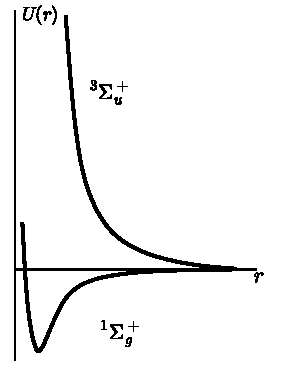
\includegraphics[width=6cm]{fig29.pdf}\\[0.3em]{\small 图 29}\end{minipage}\par\nopagebreak

因此在基态中，氢分子的总自旋 $S=0$.我们发现，差不多所有由主族元素组成的化学性质稳定的化合物的分子都具有这种性质.在无机分子中，例外的有双原子分子 $\mathrm{O}_2$（基态为 $^3\Sigma$）和 NO（基态为 $^2\Pi$）以及三原子分子 $\mathrm{NO}_2$，$\mathrm{ClO}_2$（总自旋 $S=\frac{1}{2}$）.过渡族元素具有特殊的性质，我们将在讨论了主族元素的原子价性质以后再去讨论它.

原子相互结合的性质因而和它们的自旋有关（W.~Heitler, H.~London, 1927）.进行结合时，原子的自旋相互抵消.我们最好用一个整数，即原子自旋的两倍，作为原子结合能力的定量标志.这个整数就等于该原子的化学价.在此我们必须记住，同一原子可以具有不同的原子价，要看它处于哪个态中.

让我们用这个观点看一下周期表中的主族元素.第一族元素（表3的第一列，碱金属族）的正常态中自旋为 $S=\frac{1}{2}$，因而它们的原子价等于1.只有把满壳层中的电子激发出来以后才能得到自旋值较高的激发态.但这种激发态高到这样的地步，以致激发原子无法组成稳定的分子.\footnote{关于 Cu, Ag, Au 元素，见本节末.}

第二族元素（表3第二列，碱土金属族）的原子在正常态具有 $S=0$ 的自旋.因而这些原子处于正常态时不能组成化合物.但有一个激发态比较接近于基态，它的组态不是 $\mathrm{s}^2$ 而是未满壳层中的 $\mathrm{sp}$ 组态，具有总自旋 $S=1$.处于这种态中的原子是2价的，这是第二族元素的主原子价.

第三族元素的正常态具有电子组态 $\mathrm{s}^2\mathrm{p}$ 并且自旋 $S=\frac{1}{2}$.但把封闭 $\mathrm{s}$ 壳层中的一个电子激发以后，可以得到一个激发态，它具有组态 $\mathrm{sp}^2$ 并具有自旋 $S=\frac{3}{2}$，这个态接近于正常态.因此这一族元素可以有3价和1价.此族的前两个元素（硼、铝）只表现为3价元素.随着原子序的增大，原子价为1的趋势就逐渐显示出来，铊元素表现为3价和1价的机会相等（例如在化合物 TlCl 和 $\mathrm{TlCl}_3$ 中）.这是因为对前几个元素讲来，三价化合物中的结合能大于单价化合物中的结合能，它们之间的差值超过了该原子的激发能量.

第四族元素中，基态具有组态 $\mathrm{s}^2\mathrm{p}^2$，自旋等于1，它的邻近激发态具有组态 $\mathrm{sp}^3$ 而自旋等于2.这些态相当于2价和4价.它和第三族一样，前两个元素（碳，硅）主要表现为高原子价（例如CO等为例外），随着原子序的增大而显示出低价趋势.

第五族元素的原子中，基态具有组态 $\mathrm{s}^2\mathrm{p}^3$，自旋为 $S=\frac{3}{2}$，所以相应的原子价等于3.只有把其中的一个电子激发到主量子数更高的壳层中才能得到自旋更高的激发态.这些态中最邻近的态具有组态 $\mathrm{s}^2\mathrm{p}^2\mathrm{s}'$ 并且自旋 $S=\frac{5}{2}$（我们习惯地用 $\mathrm{s}'$ 代表电子的一个 $\mathrm{s}$ 态，它的主量子数要比前一个 $\mathrm{s}$ 态大1）.这个态的激发能量虽然比较高，但是这样的激发原子仍能组成稳定的化合物.因此第五族元素表现为3价和5价（例如氮在 $\mathrm{NH}_3$ 中为3价在 $\mathrm{HNO}_3$ 中为5价）.

第六族的元素中，基态（组态为 $\mathrm{s}^2\mathrm{p}^4$）的自旋等于1，因而原子是2价的.激发一个 $\mathrm{p}$ 电子后得到自旋为2的 $\mathrm{s}^2\mathrm{p}^3\mathrm{s}'$ 态，再激发一个 $\mathrm{s}$ 电子后得到自旋为3的 $\mathrm{sp}^3\mathrm{s}'\mathrm{p}'$ 态.处于这两种激发态中的原子都能组成稳定分子，因而表现出4价和6价.第六族中的第一个元素（氧）只表现为2价，后面的一些元素把高原子价也表现出来（例如硫在 $\mathrm{H}_2\mathrm{S}$，$\mathrm{SO}_2$，$\mathrm{SO}_3$ 中分别为2,4,6价）.

第七族（卤素族）中，基态（组态 $\mathrm{s}^2\mathrm{p}^5$，自旋 $S=\frac{1}{2}$）原子是单价的.但是以下的激发态可以形成稳定化合物，这些激发态的组态分别为 $\mathrm{s}^2\mathrm{p}^4\mathrm{s}'$，$\mathrm{s}^2\mathrm{p}^3\mathrm{s}'\mathrm{p}'$，$\mathrm{sp}^3\mathrm{s}'\mathrm{p}'^2$，自旋分别为 $\frac{3}{2}$，$\frac{5}{2}$，$\frac{7}{2}$，因此原子价为3,5,7.此族的第一个元素（氟）总是单价的，但是以后的元素还表现出高原子价（例如氯在 HCl，$\mathrm{HClO}_2$，$\mathrm{HClO}_3$，$\mathrm{HClO}_4$ 中分别为1,3,5,7价）.

最后是惰性气体族元素的原子，其基态是完全封闭的壳层（因而自旋 $S=0$），它们的激发能量非常高.因此原子价等于零，这些元素在化学上是惰性的\footnote{其中某些元素仍能与氟和氧结合成稳定化合物.它们的原子价可能与封闭壳层的最外层中的电子跃迁到能量较近的未满 f 态或 d 态中有关.\par 还可以提及惰性气体原子与该元素的激发原子相互作用时所产生的相吸效应.这种效应来自处于不同状态的相同原子靠拢时可能态数的加倍（见 §80）.在这里，激发态在两个原子之间的交替跃迁作用代替了产生通常原子价的交换作用.$\mathrm{He}_2$ 分子就是这种分子的一个例子.由两个相同原子所组成的电离分子中也出现这种类型的化学键（例如 $\mathrm{H}_2^+$）.}.

以上所作的论述需要给予如下总的说明.当我们讲到分子中的一个原子具有某一激发态的原子价时，并不意味着把这个原子拉到远距离处以后一定能得到一个激发原子.它只是意味着这个分子中的电荷密度分布在该原子的原子核附近接近于一个孤立激发原子的电荷密度分布.但当原子核之间的距离增大时，这种电荷密度分布很有可能趋于非激发原子的情形.

当原子结合成为分子时，原子中的封闭电子壳层改变得很少.可是未满壳层中的电子密度分布可能会有很大的改变.在表现得最明显的异极键情形下，所有的价电子都从原来的原子跑到了另一个原子，以致我们可以把这个分子说成是由电荷（以 $e$ 为单位）等于其原子价的离子所组成.第一族的元素是正电性的：它们在异极化合物中失去电子而构成正的离子.当我们转向随后的几族时，元素的正电性逐渐不明显并转变为负电性，并在第七族元素中达到最高程度.关于异极性问题，我们需要和分子中的激发原子一样作出同样的说明.如果一个分子是异极性的，它并不意味着原子拉开后一定能得到两个离子.例如，对 CsF 分子的确可以得到 $\mathrm{Cs}^+$ 和 $\mathrm{F}^-$ 离子.但对 NaF 分子所得的却是 Na 和 F 的中性原子（因为氟的电子亲和势大于铯的电离势而小于钠的电离势）.

相反的极端情形是同极键，同极分子中的各个原子平均说来保持为中性.同极分子不同于异极分子，它并没有显著的偶极矩.异极型和同极型的区别完全是定性的，任何中间类型都有可能出现.

现在来讲过渡族元素.钯族和铂族在原子价的性质方面与主族元素极为相似.唯一不同的是，由于原子内的 d 电子处于较深的位置，它们和分子中的其它原子的作用很弱.结果使这些元素的化合物中常常出现“不饱和”的化合物，它们的分子具有不等于零的自旋（实际上都不超过 $\frac{1}{2}$）.每一种元素都可以呈现出好几种原子价，这些原子价之间的差值可以等于1，不像主族元素那样只能相差2（主族元素的原子价改变是由于电子的激发，这些激发电子的自旋原来是成对抵消的，因此激发以后有一对电子的自旋同时获得释放）.

稀土族元素是以存在未满 f 电子壳层为特征的.这些 f 电子处于比 d 电子更深的位置，因而它们并不参与原子价.所以稀土族元素的原子价只由未满壳层中的 s 和 p 电子所决定\footnote{某些稀土族原子的未满壳层中存在着 d 电子，这种电子并不重要，因为这些原子参与化合物时实际上总是处于没有 d 电子的激发态.}.但是必须注意，当原子受激以后 f 电子有可能转入 s 和 p 态，使原子价增加1.因此稀土族元素所表现的原子价其差值也等于1（实际上它们都是三价和四价的）.

锕族元素占有特殊的地位.锕和钍不含 f 电子，参与它们原子价的是 d 电子，因此它们的化学性质不像稀土元素而像钯族和铂族元素.至于铀，虽在基态中有 f 电子，但在化合物中也没有 f 电子.最后，Np，Pu，Am，Cm 原子的化合物中虽有 f 电子，但是参与原子价的电子仍为 s 和 d 电子.在这种意义下，它们都是类铀的.“未配对”的 s 和 d 电子的最大数目分别等于1和5，所以锕族元素的最高原子价等于6，而稀土族元素的最高原子价（有 s 和 p 电子参与的原子价）等于 $1+3=4$.

铁族元素，就它们的原子价性质来说，介于稀土元素与钯族铂族元素之间.这些原子中的 d 电子处于比较深的位置，在许多化合物中它们对原子价键没有贡献.因此在这样的化合物中，铁族元素类似于稀土元素.在这一类化合物中，有离子型的化合物（例如 $\mathrm{FeCl}_2$，$\mathrm{FeCl}_3$），其中的金属原子是一个阳离子.和稀土元素一样，这些化合物中的铁族元素可以有好几种原子价.

铁族元素的另一类化合物称为络合物，这类化合物的特点是分子中的过渡族元素不是一个简单的离子而是一个复合离子中的一部分（例如 $\mathrm{KMnO}_4$ 中的 $\mathrm{MnO}_4^-$ 离子，$\mathrm{K}_4\mathrm{Fe}(\mathrm{CN})_6$ 中的 $\mathrm{Fe}(\mathrm{CN})_6^{----}$ 离子）.这类复合离子中的原子要比简单离子型化合物中的原子挨得更近，在原子中 d 电子也参与了价键.因此络合物中的铁族元素类似于钯族和铂族.

最后必须提一下铜，银，金等元素，它们在§73中放在主族元素内，但在某些化合物中它们类似于过渡族元素.这些元素中，由于 d 壳层的电子可以跃迁到能量相近的 p 壳层（例如铜中的3d电子跃迁到4p），原子价可以超过1.在这样的化合物中，原子具有未满 d 壳层因而类似于过渡族：铜类似于铁族元素，银和金类似于钯族和铂族.

\begin{xiti}

基态氢原子和 $\mathrm{H}^+$ 离子结合成电离分子 $\mathrm{H}_2^+$，试求核距 $R$ 远大于玻尔半径时 $\mathrm{H}_2^+$ 的电子谱项（Л.~Д.~Ландау, 1961; C.~Herring, 1961）\footnote{关于 $\mathrm{H}_2$ 分子的相应问题，见 Л.~П.~Горьков, Л.~П.~Питаевский, ДАН СССР. 1963. Т.~151. С.~822；C.~Herring, M.~Flicker. Physical Review. \textbf{134A}, 362, 1964（第二篇文章改正了第一篇的计算错误）.}.

解：本题形式上类似于§50题3，在这里对原子核连线具有轴对称性的两个三维势阱（围绕两个核）代替了两个一维势阱.$E_0=-\frac{1}{2}$ 能级\footnote{本题采用原子单位.}（氢原子的基态能级）分裂成为 $U_g(R)$ 和 $U_u(R)$ 两个能级（$^2\Sigma_g^+$ 谱项和 $^2\Sigma_u^+$ 谱项），相应的电子波函数为
\begin{equation*}
  \psi_{g,u}(x,y,z)=\frac{1}{\sqrt{2}}\left[\psi_0(x,y,z)\pm\psi_0(-x,y,z)\right].
\end{equation*}
它们对称和反对称于平分原子核连线的 $x=0$ 平面（两核在 $x$ 轴上的 $x=\pm\frac{1}{2}R$ 点）.其中的 $\psi_0(x,y,z)$ 是一个势阱中的电子波函数.与§50题3的做法完全类似，可得
\setcounter{equation}{0}\renewcommand{\theequation}{\arabic{equation}}%
\begin{equation}
  U_{g,u}(R)-E_0=\mp\iint\psi_0\frac{\partial\psi_0}{\partial x}\,\mathrm{d}y\,\mathrm{d}z.
\end{equation}
式中的积分是对 $x=0$ 平面进行的\footnote{注意所求的效应取决于这样的距离范围，在此范围内电子以同样方式和两核作用.}.

取 $\psi_0$ 函数（设绕核1运动，该核在 $x=\frac{1}{2}R$ 处）的形式为
\begin{equation}
  \psi_0=\frac{a}{\sqrt{\pi}}\,\mathrm{e}^{-r_1},
\end{equation}
其中的 $a$ 是一个缓变函数（对氢原子，$a=1$）.$\psi_0$ 函数必须满足下列薛定谔方程
\begin{equation}
  \frac{1}{2}\nabla^2\psi+\left(-\frac{1}{2}-\frac{1}{R}
  +\frac{1}{r_1}+\frac{1}{r_2}\right)\psi=0,
\end{equation}
$r_1$ 和 $r_2$ 是电子离核1和核2的距离.这个方程中的电子总能量等于
\begin{equation*}
  E_0-\frac{1}{R},
\end{equation*}
因为 $E_0$ 本身含有原子核的库仑排斥能 $1/R$.

由于 $\psi_0$ 函数离开 $x$ 轴时很快衰减，只有远小于 $R$ 的 $y$ 和 $z$ 区域对积分式(1)才是重要的.当 $y,z\ll R$ 时，把(2)代入(3)得
\begin{equation*}
  \frac{\partial a}{\partial x}+\frac{a}{\frac{1}{2}R+x}-\frac{a}{R}=0.
\end{equation*}
式中略去了缓变函数 $a$ 的二阶导数并已令 $r_2\approx\frac{1}{2}R+x$.上式中 $x\to\frac{1}{2}R$（即在核1邻区）时等于1的解为
\begin{equation*}
  a=\frac{2R}{R+2x}\exp\left(\frac{x}{R}-\frac{1}{2}\right).
\end{equation*}
这时(1)式给出
\begin{equation*}
  U_{g,u}-E_0=\mp\frac{4}{\pi e}\int_{R/2}^{\infty}\mathrm{e}^{-2r_1}2\pi r_1\,\mathrm{d}r_1
  =\mp2R\,\mathrm{e}^{-R-1},
\end{equation*}
分裂量为\footnote{按前引文献，$\mathrm{H}_2$ 分子的相应结果为 $U_g-U_u=-1.64R^{5/2}\,\mathrm{e}^{-2R}$.}
\begin{equation}
  U_g-U_u=-4R\,\mathrm{e}^{-R-1}.
\end{equation}
在足够远的距离处，这个表示式指数式地衰减到小于 H 原子与 $\mathrm{H}^+$ 离子偶极矩相互作用的二级近似效应.由于基态氢原子的极化率等于9/2［见(77.9)］，而 $\mathrm{H}^+$ 离子的场为 $\mathcal{E}=1/R^2$，相应的相互作用能等于 $-9/(4R^4)$，计及此式后得
\begin{equation}
  U_{g,u}(R)-E_0=\mp\frac{2}{e}R\,\mathrm{e}^{-R}-\frac{9}{4R^4}.
\end{equation}
仅当 $R=10.8$ 时第二项才能与第一项差不多.我们还要指出，$U_u$ 谱项在 $R=12.6$ 处具有一个极小值，它等于 $-5.8\times10^{-5}$ 原子单位（$-1.6\times10^{-3}\,\mathrm{eV}$）\footnote{这个极小值来自范德瓦尔斯力，它和稳定离子 $\mathrm{H}_2^+$ 的基态谱项 $U_g(R)$ 的极小值相比是极浅的：后一个极小值为 $-0.6$ 原子单位（$-16.3\,\mathrm{eV}$），位于 $R=2.0$ 处.}.

\end{xiti}
\renewcommand{\theequation}{\arabic{section}.\arabic{equation}}%

\section{双原子分子单重谱项的振动和转动结构}

正如本章初所指出的，核质量与电子质量的巨大差别，使我们有可能把确定分子能级的问题分成两个部分.我们先求原子核为静止时的多电子系统的能级，作为核距的函数（电子谱项）.然后可以考虑对一个给定电子态而言的核运动，这相当于把核看作是按 $U_n(r)$ 规律相互作用着的一组粒子，$U_n$ 是相应的电子谱项.分子的运动是由整体平动以及原子核绕质心的运动合成的.我们对整体平动当然不感兴趣，可把质心看作是固定的.

为讨论方便计，我们首先考虑分子总自旋 $S$ 为零的电子谱项（单项）.按 $U(r)$ 规律作用着的两体（两个核）相对运动问题可以化成质量为 $M$（两粒子的折合质量）的一个单粒子在一有心力场 $U(r)$ 中的运动.$U(r)$ 就是所考虑电子谱项的能量.有心力场 $U(r)$ 中的运动问题又可以化成势场中的一维运动问题，该势场的有效能量等于 $U(r)$ 与离心能之和.

我们令 $\boldsymbol{K}$ 为分子的总角动量，它由电子的轨道角动量 $\boldsymbol{L}$ 和原子核的转动角动量相加而成.于是原子核的离心能算符可写成
\begin{equation*}
  B(r)(\hat{\boldsymbol{K}}-\hat{\boldsymbol{L}})^2.
\end{equation*}
我们引用了双原子分子理论中习用的记号：
\begin{equation}
  B(r)=\frac{\hbar^2}{2Mr^2},
\end{equation}
这个算符对电子态（$r$ 为给定）平均以后，所得的离心能是 $r$ 的函数，它出现于有效势能 $U_K(r)$ 的表式中：
\begin{equation}
  U_K(r)=U(r)+B(r)\overline{(\boldsymbol{K}-\boldsymbol{L})^2},
\end{equation}
式中的横线代表上述平均.

我们来算出对某个态的平均值，该态中分子的总角动量平方具有定值 $\boldsymbol{K}^2=K(K+1)$（式中 $K$ 为整数），同时电子角动量沿分子轴（$z$ 轴）的分量具有定值 $L_z=\Lambda$.展开(82.2)式的括号，我们有
\begin{equation}
  U_K(r)=U(r)+B(r)K(K+1)-2B(r)\overline{\boldsymbol{L}}\cdot\boldsymbol{K}
  +B(r)\overline{L^2},
\end{equation}
最后一项不含量子数 $K$ 而只与电子态有关，它可以合并到能量 $U(r)$ 中去.我们来证明这一点对其前一项也是成立的.

§27末表明，如果角动量沿某轴的分量具有定值，则角动量矢量的平均值也沿该轴.如令 $\boldsymbol{n}$ 为沿 $z$ 轴的单位矢量，则有 $\overline{\boldsymbol{L}}=\Lambda\boldsymbol{n}$.经典力学中，双粒子（例如原子核）系统的转动角动量为 $\boldsymbol{r}\times\boldsymbol{p}$，其中 $\boldsymbol{r}=r\boldsymbol{n}$ 是双粒子之间的径矢，$\boldsymbol{p}$ 是相对运动的动量.这个角动量垂直于 $\boldsymbol{n}$.量子力学中，这一点对原子核的转动角动量算符同样成立：
$(\hat{\boldsymbol{K}}-\hat{\boldsymbol{L}})\cdot\boldsymbol{n}=0$，或 $\hat{\boldsymbol{K}}\cdot\boldsymbol{n}=\hat{\boldsymbol{L}}\cdot\boldsymbol{n}$.这两个算符相等，它们的本征值当然也相等，又由于 $\boldsymbol{n}\cdot\boldsymbol{L}=L_z=\Lambda$，我们有
\begin{equation}
  \boldsymbol{K}\cdot\boldsymbol{n}=\Lambda,
\end{equation}
因此(82.3)式的最后第二项为 $\overline{\boldsymbol{L}}\cdot\boldsymbol{K}=\boldsymbol{n}\cdot\boldsymbol{K}\,\Lambda=\Lambda^2$，它与 $K$ 无关.重新定义 $U(r)$ 函数，可把有效势能最后写成
\begin{equation}
  U_K(r)=U(r)+B(r)K(K+1).
\end{equation}
由公式 $K_z=\Lambda$ 可知，给定 $\Lambda$ 值后，量子数 $K$ 的取值只能是
\begin{equation}
  K\geqslant\Lambda.
\end{equation}
求解具有(82.5)式势能的一维薛定谔方程，可得一组能级.我们把这些能级（具有同一 $K$ 值的能级）按能量的递增次序加以编号，编号数为 $v=0,1,2,\cdots$；$v=0$ 对应于最低能级.由此可见，核运动使每个电子谱项分裂成为一组能级，用 $K$ 和 $v$ 两个量子数加以标志.

这些能级（对一个给定的电子谱项）的总数可以是有限的或无限的.如果电子态是这样的，即当 $r\to\infty$ 时该分子变成两个孤立的中性原子，那么势能 $U(r)$［因而还有 $U_K(r)$］在 $r\to\infty$ 时要比 $1/r$ 趋于零更快地趋于某一极限常数值 $U(\infty)$（两个孤立原子能量之和，见§89）.在这样的场中，能级数是有限的（见§18），尽管在实际分子中这个能级数是一个很大的数值.这些能级是这样分布的，即对任一给定的 $K$ 值而言，能级数具有一定的数值（它们的 $v$ 值不同），当 $K$ 增大时具有同一 $K$ 值的能级数减少，直到某一 $K$ 值根本不存在能级为止.

另一方面，如果 $r\to\infty$ 时分子分解成两个离子，则在远距离处，$U(r)-U(\infty)$ 变成按库仑定律（$\sim1/r$）吸引的离子吸引能.在这样的场中有无穷多个能级，愈来愈密地挤向极限值 $U(\infty)$.可以指出，对大多数基态分子讲来都属于前一种情形，只有相当少数的分子当原子核离远后变成一对离子.

我们不能完整地算出能级依赖于量子数的一般表式.这样的计算只有对离基态不太远的那些低激发态才是可能的\footnote{我们总是指属于同一电子谱项的那些能级.}.这些能级所对应的 $K$ 和 $v$ 量子数都很小.实际上，分子光谱研究中经常考虑的也就是这些能级，因此我们对它们特别感兴趣.

低激发态中的核运动可以看成平衡位置附近的小振动.据此我们可以把 $U(r)$ 展成 $\xi=r-r_e$ 的幂级数，$r_e$ 等于 $U(r)$ 取极小值时的 $r$ 值.由于 $U'(r_e)=0$，展到二次项为止时我们有
\begin{equation*}
  U(r)=U_e+\frac{1}{2}M\omega_e^2\xi^2,
\end{equation*}
其中 $U_e=U(r_e)$，$\omega_e$ 是振动频率.

(82.5)式右边第二项（离心能）中只要令 $r=r_e$ 就足够了，因为该项中已经含有小量 $K(K+1)$.因而有
\begin{equation}
  U_K(r)=U_e+B_eK(K+1)+\frac{1}{2}M\omega_e^2\xi^2,
\end{equation}
其中的 $B_e=\hbar^2/(2Mr_e^2)=\hbar^2/(2I)$ 称为转动常数（$I=Mr_e^2$ 是该分子的转动惯量）.

(82.7)式的前两项都是常数，第三项相当于一维谐振子.因此我们可以立刻写出所求的能级：
\begin{equation}
  E=U_e+B_eK(K+1)+\hbar\omega_e\left(v+\frac{1}{2}\right).
\end{equation}
可见在上述近似下，能级由三个独立部分所组成：
\begin{equation}
  E=E_{\mathrm{el}}+E_r+E_v,
\end{equation}
第一项 $E_{\mathrm{el}}=U_e$ 是电子能量（包括相距为 $r=r_e$ 的原子核库仑能），第二项为
\begin{equation}
  E_r=B_eK(K+1),
\end{equation}
这是分子转动\footnote{描述双原子分子（无自旋）转动的波函数基本上和一个对称陀螺（§103）相同.与陀螺不同之处是，分子的转动只需用定义分子轴线方向的两个角度（$\alpha\equiv\varphi$，$\beta\equiv\theta$）来描写，转动波函数与（103.8）式不同之处在于量子数的记号并且少了一个 $\mathrm{e}^{\mathrm{i}k\gamma}/\sqrt{2\pi}$ 因子.按（82.4）式，$\Lambda$ 是总角动量 $K$ 沿分子轴（§103 中的 $\zeta$ 轴）的分量，我们必须用 $K$，$M$ 和 $\Lambda$（这里 $M=K_\zeta$）代替 $J$，$M$ 和 $k$.因此
\begin{equation*}
  \psi_{\mathrm{rot}}(\varphi,\theta)=\mathrm{i}^K\sqrt{\frac{2K+1}{4\pi}}D^{(K)}_{\Lambda M}(\varphi,\theta,0).
\end{equation*}}的转动能.第三项为
\begin{equation}
  E_v=\hbar\omega_e\left(v+\frac{1}{2}\right),
\end{equation}
它是分子内原子核的振动能.根据定义，$v$ 是具有给定 $K$ 值的那些能级按能量递增次序加以编号的编号数，称为振动量子数.

对一个形状给定的势能曲线 $U(r)$，频率 $\omega_e$ 和 $\sqrt{M}$ 成反比.因此振动能级间距 $\Delta E_v$ 和 $1/\sqrt{M}$ 成正比.转动能级间距 $\Delta E_r$ 的分母中含有转动惯量 $I$，因此和 $1/M$ 成正比.电子能级及其间距 $\Delta E_e$ 和 $M$ 无关.由于 $m/M$（$m$ 为电子质量）在双原子分子理论中是一个小参量，我们有
\begin{equation}
  \Delta E_{\mathrm{el}}\gg\Delta E_v\gg\Delta E_r,
\end{equation}
上式给出颇不寻常的分子能级分布.核振动把电子谱项分裂成为一组相靠较近的能级.这些能级又由于分子的转动而显示出精细分裂\footnote{作为例子，下面给出几个分子的 $U_e$，$\hbar\omega_e$ 和 $B_e$ 值（以 eV 为单位）
\begin{center}
\begin{tabular}{lccc}
  & $\mathrm{H}_2$ & $\mathrm{N}_2$ & $\mathrm{O}_2$ \\
  $-U_e$ & 4.7 & 7.5 & 5.2 \\
  $\hbar\omega_e$ & 0.54 & 0.29 & 0.20 \\
  $10^3\times B_e$ & 7.6 & 0.25 & 0.18
\end{tabular}
\end{center}}.

下一级近似中，能量不再能分成振动和转动两个独立部分；出现了同时含有 $K$ 和 $v$ 的转动–振动项.计算逐级近似后，所得的 $E$ 是量子数 $K$ 和 $v$ 的一个幂级数展式.

我们将在这里计算(82.8)式的下一级近似.为此，我们必须把 $U(r)$ 展开至 $\xi$ 的四次幂为止（参考§38中的非谐振子问题）.同样地，离心能也要展至 $\xi^2$ 项.这样得到
\begin{equation}
\begin{aligned}
  U_K(r)={}&U_e+\frac{1}{2}M\omega_e^2\xi^2+\frac{\hbar^2}{2Mr_e^2}K(K+1)-a\xi^3+b\xi^4\\
  &-\frac{\hbar^2}{Mr_e^3}K(K+1)\xi+\frac{3\hbar^2}{2Mr_e^4}K(K+1)\xi^2.
\end{aligned}
\end{equation}
现在把(82.13)中的最后四项当作微扰算符，来计算对(82.8)的本征值的改正.对于 $\xi^2$ 和 $\xi^4$ 项应用微扰论的一级近似就够了，但对 $\xi$ 和 $\xi^3$ 项一定要计算二级近似，因为 $\xi$ 和 $\xi^3$ 的对角矩阵元都等于零.所有要计算的矩阵元都已在§23和§38题3中导出.所得的结果通常表成下列形式：
\begin{equation}
\begin{aligned}
  E={}&E_{\mathrm{el}}+\hbar\omega_e\left(v+\frac{1}{2}\right)
  -x_e\hbar\omega_e\left(v+\frac{1}{2}\right)^2+B_vK(K+1)\\
  &-D_eK^2(K+1)^2,
\end{aligned}
\end{equation}
其中的
\begin{equation}
  B_v=B_e-\alpha_e\left(v+\frac{1}{2}\right)\equiv B_0-\alpha_ev.
\end{equation}
$x_e$，$B_e$，$\alpha_e$，$D_e$ 等常数与(82.13)式中的常数有以下关系：
\begin{equation}
\begin{aligned}
  B_e&=\frac{\hbar^2}{2I},\qquad D_e=\frac{4B_e^3}{\hbar^2\omega_e^2},\\
  \alpha_e&=\frac{6B_e^2}{\hbar\omega_e}
  \left(\frac{a\hbar}{M\omega_e^2}\sqrt{\frac{2}{MB_e}}-1\right),\\
  x_e&=\frac{3}{2\hbar\omega_e}\left(\frac{\hbar}{M\omega_e}\right)^2
  \left[\frac{5}{2}\frac{a^2}{M\omega_e^2}-b\right].
\end{aligned}
\end{equation}
和 $v,K$ 无关之项已归在 $E_{\mathrm{el}}$ 内.

\begin{xiti}

把双原子分子中的电子运动和核运动分离开来，试确定这种近似的准确程度.

解：分子总哈密顿量可写成 $\hat{H}=\hat{T}_r+\hat{H}_{\mathrm{el}}$，其中 $\hat{T}_r=\hat{\boldsymbol{p}}^2/2M$ 是原子核相对运动的动能算符（$\hat{\boldsymbol{p}}=-\mathrm{i}\hbar\partial/\partial\boldsymbol{r}$；$\boldsymbol{r}$ 是连结原子核的径矢；$M$ 是折合质量）.哈密顿量 $\hat{H}_{\mathrm{el}}$ 中包括电子的动能算符、电子之间以及电子与原子核之间的库仑势能和原子核之间的库仑能\footnote{哈密顿量 $\hat{H}$ 取的是分子质心为静止的坐标系（$\boldsymbol{P}_{\mathrm{n}}+\boldsymbol{P}_{\mathrm{e}}=0$，$\boldsymbol{P}_{\mathrm{n}}$ 是两个核的总动量，$\boldsymbol{P}_{\mathrm{e}}$ 是电子总动量）.其中没有包含质心动能 $\boldsymbol{P}_{\mathrm{n}}^2/2(M_1+M_2)=\boldsymbol{P}_{\parallel}/2(M_1+M_2)$，与电子动能相比，这一项确实很小，比例为 $m/M$.}.设薛定谔方程
\setcounter{equation}{0}\renewcommand{\theequation}{\arabic{equation}}%
\begin{equation}
  \hat{H}\psi=(\hat{T}_r+\hat{H}_{\mathrm{el}})\psi=E\psi
\end{equation}
之解的形式为
\begin{equation}
  \psi=\sum_m{}'\chi_m(\boldsymbol{r})\varphi_m(q,\boldsymbol{r})
\end{equation}
其中的函数组 $\varphi_m(q,\boldsymbol{r})$ 是下列方程的正交归一化解：
\begin{equation}
  \hat{H}_{\mathrm{el}}\varphi_m(q,\boldsymbol{r})=U_m(\boldsymbol{r})\varphi_m(q,\boldsymbol{r}).
\end{equation}
$q$ 代表电子坐标全体；$U_m(\boldsymbol{r})$ 是哈密顿量 $\hat{H}_{\mathrm{el}}$ 的本征值，它依赖于参量 $\boldsymbol{r}$.把(2)代入(1)，乘以 $\varphi_n^*(q,\boldsymbol{r})$ 并对 $q$ 积分，得
\begin{equation}
  \left[\frac{\hat{\boldsymbol{p}}^2}{2M}+V_{nn}''+U_n(\boldsymbol{r})-E\right]\chi_n(\boldsymbol{r})
  =-\sum_m{}'\bigl(\hat{V}_{nm}'+V_{nm}''\bigr)\chi_m(\boldsymbol{r}),
\end{equation}
其中
\begin{equation*}
  \hat{V}_{nm}'=\frac{1}{M}\boldsymbol{p}_{nm}\cdot\hat{\boldsymbol{p}},\qquad
  V_{nm}''=\frac{1}{2M}(\boldsymbol{p}^2)_{nm}.
\end{equation*}
而 $\boldsymbol{p}_{nm}=\int\varphi_n^*\hat{\boldsymbol{p}}\varphi_m\,\mathrm{d}q$，$(\boldsymbol{p}^2)_{nm}$ 是对电子波函数而言的矩阵元，对角元 $\boldsymbol{p}_{nn}$ 由于对称性而等于零.

电子波函数 $\varphi_n$ 只是在原子尺度内变化显著，它们对 $\boldsymbol{r}$ 的微商不会引进大的 $M/m$ 参量（$m$ 为电子质量）.因而 $V_{nn}''$ 与 $U_n(\boldsymbol{r})$ 相比小 $m/M$ 倍，可以略去.如果把(4)式右边看作一个小的微扰，则零级近似波函数 $\chi_n(\boldsymbol{r})$ 为下式之解：
\begin{equation}
  \left[\frac{\hat{\boldsymbol{p}}^2}{2M}+U_n(\boldsymbol{r})\right]\chi_{nv}=E_{nv}\chi_{nv}.
\end{equation}
上式描述 $U_n(\boldsymbol{r})$ 场中的核运动（$v$ 是这种运动的量子数）.微扰论的适用条件是
\begin{equation*}
  \left|\langle nv'|\hat{V}_{nm}'+V_{nm}''|mv\rangle\right|
  \ll\left|E_{nv'}-E_{mv}\right|.
\end{equation*}
不等式的右边是不同电子谱项的能量差，此量对小的 $m/M$ 参量而言为零级.式左边含有核波函数的矩阵元.$V_{nm}''$ 中含有 $m/M$ 因子，它确是很小.在 $\hat{V}_{nm}'$ 的矩阵元中，算符 $\hat{\boldsymbol{p}}$ 作用于 $\chi_{mv}$ 函数，使它乘上了一个核动量的数量级的量.如果原子核作小振动，其动量 $\sim\sqrt{M\hbar\omega_e}$；由于频率 $\omega_e$ 和 $\sqrt{M}$ 成反比，矩阵元 $\langle nv'|\hat{V}_{nm}'|mv\rangle$ 为 $(m/M)^{3/4}$ 数量级.

\end{xiti}
\renewcommand{\theequation}{\arabic{section}.\arabic{equation}}%

\section{多重谱项·情形\texorpdfstring{$a$}{a}}

现在来研究自旋 $S$ 不等于零的分子能级的分类问题.在零级近似中，当相对论效应完全略去以后，分子和任意多粒子系统一样，它的能量与自旋的方向无关（此自旋是“自由”的），结果使能级具有 $(2S+1)$ 重简并.但当考虑了相对论效应以后，能级就会分裂，从而使能量成为自旋沿分子轴方向的投影值的函数.我们将把分子中的相对论作用称为自旋–轴作用.它的主要部分（和原子的情形一样）就是自旋和电子轨道运动间的相互作用\footnote{除了自旋–轨道作用和自旋–自旋作用以外，还有分子转动与电子自旋及轨道运动间的相互作用.但是这一部分的作用很小，可能只对自旋 $S=\frac{1}{2}$ 的谱项有意义（见 §84）.}.

分子能级的性质及其分类，明显地依赖于自旋轨道作用和分子转动两者的相对重要性.后者所起的作用可以拿两个相邻转动能级的间距作标志.与此相应，我们来考虑两种极端情形.一种情形是自旋–轴作用的能量大于转动能级之间的能量差，另一种情形则相反.第一种情形通常称为情形$a$（或 $a$ 型耦合），第二种情形称为情形$b$（F.~Hund, 1933）.

情形$a$最为常见.$\Sigma$ 谱项是一个例外，其中主要属于情形$b$，因为自旋–轴作用效应对这种谱项讲来是很小的（见后）\footnote{一个特殊情形是 $\mathrm{O}_2$ 分子的电子基项（$^3\Sigma$ 谱项）.它的耦合情况介于 $a$ 型和 $b$ 型之间（见 §84 题 3）.}.对于其它的谱项讲来，情形$b$有时在极轻的分子中见到，因为这种情形下的自旋–轴作用比较弱，而转动能级的间距比较大（转动惯量比较小）.

介于 $a$ 和 $b$ 之间的中间情形当然也是可能的.还必须注意到，同一个电子态当转动量子数改变时可以从情形$a$连续地变到情形$b$.原因在于，相邻转动能级之间的间距是随着转动量子数的增大而增大的，因此即使在较低转动能级时属于情形$a$，但当转动量子数增大后，转动能级间距就有可能大于自旋–轴作用的耦合能量（情形$b$）.

情形$a$的能级分类原则上与自旋为零的谱项分类没有多大的区别.我们首先考虑原子核静止时亦即完全略去转动时的电子谱项.除了电子轨道角动量的投影值 $\Lambda$ 以外，现在还必须考虑总自旋沿分子轴的投影值，我们用 $\Sigma$ 代表这个投影量\footnote{不要和 $\Lambda=0$ 的谱项符号混淆起来！}，它的取值为 $S,S-1,\cdots,-S$.当自旋和轨道角动量在分子轴上的投影方向一致时，我们令 $\Sigma$ 取正值（注意 $\Lambda$ 代表轨道角动量投影值的绝对值）.$\Lambda$ 和 $\Sigma$ 相加起来给出沿分子轴的电子总角动量：
\begin{equation}
  \Omega=\Lambda+\Sigma;
\end{equation}
它的取值为 $\Lambda+S,\Lambda+S-1,\cdots,\Lambda-S$.由此可见，轨道角动量为 $\Lambda$ 的一个电子谱项分裂成为 $2S+1$ 个具有不同 $\Omega$ 值的谱项；和原子谱项的情形一样，我们把这种分裂称为该电子能级的精细结构或多重分裂.通常把 $\Omega$ 值标在谱项符号的右下角；例如 $\Lambda=1$，$S=\frac{1}{2}$ 时我们得到 $^2\Pi_{1/2}$，$^2\Pi_{3/2}$ 两个谱项.

考虑了原子核的运动以后，每一个这样的谱项中会出现振动和转动结构.各种转动能级是用分子总角动量量子数 $J$ 的数值来标志的，这个总角动量包括了电子的自旋和轨道角动量以及原子核的转动角动量\footnote{符号 $K$ 仍保留为不考虑自旋时的分子总角动量.情形 $a$ 中量子数 $K$ 并不存在.因为角动量 $K$ 即使近似地讲来也不能守恒.}.$J$ 可以取从 $|\Omega|$ 值开始的各种整数值：
\begin{equation}
  J\geqslant|\Omega|,
\end{equation}
显然这是(82.6)式的推广.

现在来推导情形$a$中分子能级的定量公式.先考虑电子谱项的精细结构.我们在§72中讨论原子谱项的精细结构时应用了(72.4)式，该式表明自旋–轨道作用的平均值与原子总自旋沿轨道角动量矢量方向的投影值成正比.与此完全类似，双原子分子中的自旋–轴作用（对原子核间距给定为 $r$ 时的电子态取平均）和分子总自旋在分子轴上的投影值 $\Sigma$ 成正比，因此可把所分裂的电子谱项写成下列形式：
\begin{equation*}
  U(r)+A(r)\Sigma,
\end{equation*}
式中的 $U(r)$ 是原谱项（未分裂前的谱项）的能量，$A(r)$ 是 $r$ 的某一函数，这个函数与原谱项有关（特别是和 $\Lambda$ 值有关）但和 $\Sigma$ 无关.由于人们通常采用量子数 $\Omega$ 而不用 $\Sigma$，为方便计，我们可把 $A\Sigma$ 改成 $A\Omega$；所差的 $A\Lambda$ 可以包括在 $U(r)$ 内.因此对于一个电子谱项，我们有以下的表式
\begin{equation}
  U(r)+A(r)\Omega.
\end{equation}
注意分裂谱项的各个分量是彼此等距的：相邻分量（$\Omega$ 值相差为1）的间距与 $\Omega$ 无关并等于 $A(r)$.

根据一般考虑很易证明 $\Sigma$ 谱项的 $A$ 值等于零.为此我们来进行时间反号操作.此时的能量值一定保持不变，可是分子态中沿分子轴的自旋和轨道角动量都要反向.能量 $A(r)\Sigma$ 中的 $\Sigma$ 就要变号，如果能量保持不变，则 $A(r)$ 必须变号.如果 $\Lambda\neq0$，我们对 $A(r)$ 的数值不能作出任何结论，因为 $A(r)$ 依赖于轨道角动量，而轨道角动量本身也要变号.但当 $\Lambda=0$ 时，我们可以肯定 $A(r)$ 此时是不变的，因此它只能等于零.由此可见，对 $\Sigma$ 谱项讲来，一级近似中的自旋–轴作用并不产生能级分裂；只有考虑了二级近似中的自旋–轴作用或者是一级近似中的自旋–自旋作用以后，能级才会分裂（与 $\Sigma^2$ 成正比）但是比较小.这就是前面提到的 $\Sigma$ 谱项往往属于情形$b$的根据.

当我们求出了多重分裂以后，分子的转动就可以当作微扰来处理，完全类似于§82开始所作的推导.原子核的转动角动量可以从总角动量中减去电子的轨道角动量以及自旋以后得到，所以离心能算符现在呈下列形式：
\begin{equation*}
  B(r)(\hat{\boldsymbol{J}}-\hat{\boldsymbol{L}}-\hat{\boldsymbol{S}})^2,
\end{equation*}
上式对电子态求平均后再加到(83.3)式中，即得欲求的有效势能 $U_J(r)$：
\begin{equation*}
\begin{aligned}
  U_J(r)&=U(r)+A(r)\Omega+B(r)\overline{(\boldsymbol{J}-\boldsymbol{L}-\boldsymbol{S})^2}=\\
  &=U(r)+A(r)\Omega+B(r)\bigl[J^2-2\boldsymbol{J}\cdot\overline{(\boldsymbol{L}+\boldsymbol{S})}\\
  &\qquad+\overline{L^2}+2\overline{\boldsymbol{L}\cdot\boldsymbol{S}}+\overline{S^2}\bigr].
\end{aligned}
\end{equation*}
$J^2$ 的本征值是 $J(J+1)$.其次，根据和§82中相同的论证，我们有：
\begin{equation}
  \overline{\boldsymbol{L}}=\boldsymbol{n}\Lambda,\qquad
  \overline{\boldsymbol{S}}=\boldsymbol{n}\Sigma,
\end{equation}
还有 $(\hat{\boldsymbol{J}}-\hat{\boldsymbol{L}}-\hat{\boldsymbol{S}})\cdot\boldsymbol{n}=0$，因此有本征值：
\begin{equation}
  \boldsymbol{J}\cdot\boldsymbol{n}=(\hat{\boldsymbol{L}}+\hat{\boldsymbol{S}})\cdot\boldsymbol{n}
  =\Lambda+\Sigma=\Omega.
\end{equation}
把以上诸值代入，我们得：
\begin{equation*}
  U_J(r)=U(r)+A(r)\Omega+B(r)\bigl[J(J+1)-2\Omega^2
  +\overline{L^2}+2\overline{\boldsymbol{L}\cdot\boldsymbol{S}}+\overline{S^2}\bigr].
\end{equation*}
对电子态平均时采用的是零级近似波函数\footnote{这是既对分子转动效应又对自旋–轴作用而言的零级近似.}.但在这种近似中自旋值是守恒的，从而 $S^2=S(S+1)$.这个波函数是自旋函数和坐标函数的乘积；因此角动量 $\boldsymbol{L}$ 和 $\boldsymbol{S}$ 的平均是相互独立地进行的，我们可得
\begin{equation*}
  \overline{\boldsymbol{L}}\cdot\overline{\boldsymbol{S}}=\Lambda\boldsymbol{n}\cdot\overline{\boldsymbol{S}}=\Lambda\Sigma.
\end{equation*}
最后，轨道角动量 $L^2$ 的平均值与自旋无关，它是标志所给电子谱项（未分裂的谱项）的一个 $r$ 的函数.凡是 $r$ 的函数但与 $J$，$\Sigma$ 无关的项都可以包括在 $U(r)$ 中，凡是与 $\Sigma$（或者 $\Omega$）成正比的项都可以包括在表式 $A(r)\Omega$ 中.因此可得下列有效势能表式
\begin{equation}
  U_J(r)=U(r)+A(r)\Omega+B(r)\bigl[J(J+1)-2\Omega^2\bigr].
\end{equation}
利用§82中从(82.5)式开始的那种方法，我们可以求出目前情形下的分子能级.把 $U(r)$ 和 $A(r)$ 展为 $\xi$ 的幂级数，对 $U(r)$ 只展到 $\xi$ 的二次幂为止，但对上式中的第二项和第三项只保留零次幂，我们得到以下能级表式：
\begin{equation}
  E=U_e+A_e\Omega+\hbar\omega_e\left(v+\frac{1}{2}\right)
  +B_e\bigl[J(J+1)-2\Omega^2\bigr],
\end{equation}
式中的 $A_e=A(r_e)$ 和 $B_e$ 是标志所给（未分裂）谱项的一些常数.继续展至高次幂以后，可得含有量子数的高次幂项的一个级数，我们就不在这里写出来了.

\section{多重谱项·情形\texorpdfstring{$b$}{b}}

现在转向情形$b$.此时分子的转动效应超过了多重分裂.因此我们必须首先考虑转动效应而略去自旋–轴作用，然后把后者作为微扰来处理.

自旋为“自由”的分子中，守恒的不但有总角动量 $\boldsymbol{J}$，而且还有 $\boldsymbol{K}$（原子核角动量与电子轨道角动量之和），$\boldsymbol{K}$ 和 $\boldsymbol{J}$ 的关系为：
\begin{equation}
  \boldsymbol{J}=\boldsymbol{K}+\boldsymbol{S},
\end{equation}
量子数 $K$ 区别具有自由自旋的一个转动分子中某一给定电子谱项的各个不同态.在给定 $K$ 值的态中，有效势能 $U_K(r)$ 显然是和 $S=0$ 情形时的(82.5)式一样的：
\begin{equation}
  U_K(r)=U(r)+B(r)K(K+1),
\end{equation}
式中 $K$ 的取值为 $\Lambda,\Lambda+1,\cdots$.

考虑到自旋–轴作用以后，每一谱项一般分裂成为 $2S+1$ 个谱项（或者是 $2K+1$ 个谱项，如果 $K<S$），它们具有不同的总角动量 $J$\footnote{情形 $b$ 中，自旋沿分子轴的投影 $\boldsymbol{n}\cdot\boldsymbol{S}$ 并不具有定值，所以不存在量子数 $\Sigma$（或 $\Omega$）.}.根据角动量相加的一般法则，$J$ 的取值（当 $K$ 给定后）是从 $K+S$ 到 $|K-S|$：
\begin{equation}
  |K-S|\leqslant J\leqslant K+S.
\end{equation}
计算分裂能量（用微扰论的一级近似）时，需要求出自旋–轴作用能量算符对零级近似态（相对于自旋–轴作用的零级近似态）的平均值.在目前情形下，这意味着既对电子态又对分子转动态（$r$ 为给定）求平均.我们知道，第一个平均的结果是一个 $A(r)\boldsymbol{n}\cdot\hat{\boldsymbol{S}}$ 形式的算符，它与自旋算符沿分子轴的投影 $\boldsymbol{n}\cdot\hat{\boldsymbol{S}}$ 成正比.再把这个算符对分子转动求平均，并取自旋矢量的方向为任意，则有 $\overline{\boldsymbol{n}}\cdot\hat{\boldsymbol{S}}=\overline{\boldsymbol{n}\cdot\hat{\boldsymbol{S}}}$.平均值 $\overline{\boldsymbol{n}}$ 是一个矢量，从对称性角度考虑应该和“矢量”$\hat{\boldsymbol{K}}$ 的方向一致，$\hat{\boldsymbol{K}}$ 是标志分子转动的唯一矢量.因此可以写作
\begin{equation*}
  \overline{\boldsymbol{n}}=\text{常数}\times\hat{\boldsymbol{K}},
\end{equation*}
式中的常数很容易求出，只要以 $\hat{\boldsymbol{K}}$ 乘等式的两边并注意本征值 $\boldsymbol{n}\cdot\boldsymbol{K}=\Lambda$［见(82.4)式］及 $\boldsymbol{K}^2=K(K+1)$，即有
\begin{equation*}
  \overline{\boldsymbol{n}\cdot\hat{\boldsymbol{S}}}
  =\frac{\Lambda}{K(K+1)}\hat{\boldsymbol{K}}\cdot\hat{\boldsymbol{S}}.
\end{equation*}
最后，根据一般公式(31.3)，乘积 $\boldsymbol{K}\cdot\boldsymbol{S}$ 的本征值等于：
\begin{equation}
  \boldsymbol{K}\cdot\boldsymbol{S}
  =\frac{1}{2}\bigl[J(J+1)-K(K+1)-S(S+1)\bigr].
\end{equation}
结果，所求的自旋–轴作用能量平均值如下式所示：
\begin{equation*}
\begin{aligned}
  A(r)&\frac{\Lambda}{2K(K+1)}
  \bigl[J(J+1)-K(K+1)-S(S+1)\bigr]=\\
  ={}&A(r)\frac{\Lambda}{2K(K+1)}(J-S)(J+S+1)-\frac{1}{2}A(r)\Lambda,
\end{aligned}
\end{equation*}
这个式子应该加到(84.2)式的能量公式中.其中的 $\frac{1}{2}A(r)\Lambda$ 项与 $K$ 和 $J$ 无关可以包括在 $U(r)$ 内，因此有效势能的表式最后为
\begin{equation}
\begin{aligned}
  U_K(r)={}&U(r)+B(r)K(K+1)\\
  &+A(r)\Lambda\frac{(J-S)(J+S+1)}{2K(K+1)}.
\end{aligned}
\end{equation}
按通常方式展成 $\xi=r-r_0$ 的幂级数以后，即得情形 $b$ 时的分子能级表式：
\begin{equation}
\begin{aligned}
  E={}&U_e+\hbar\omega_e\left(v+\frac{1}{2}\right)+B_eK(K+1)\\
  &+A_e\Lambda\frac{(J-S)(J+S+1)}{2K(K+1)}.
\end{aligned}
\end{equation}
正如上节所指出的，$\Sigma$ 谱项的自旋–轴作用在一级近似下并不给出多重分裂，为了求出它的精细结构，我们有必要考虑自旋–自旋作用，它的算符是电子自旋的二次式.现在我们感兴趣的并不是这个算符本身，而是这个算符对该分子的电子态的平均结果，正如我们对自旋–轴作用算符所作的那样.显然，从对称性考虑可知，所求的平均算符应该和总自旋对分子轴的投影值的平方成正比，也就是说可以写成下列形式：
\begin{equation}
  \alpha(r)(\hat{\boldsymbol{S}}\cdot\boldsymbol{n})^2,
\end{equation}
式中的 $\alpha(r)$ 又是一个标志所给电子谱项的距离的函数.对称性的考虑中还允许存在一个与 $S^2$ 成正比的项，但由于自旋的绝对值是一个常数，这一项无关紧要.我们不打算在这里推导一个繁杂的普遍公式去说明(84.7)式的算符所产生的分裂，本节的题1中将推导出对 $\Sigma$ 三重谱项的公式.

$\Sigma$ 双重谱项是一个特殊情形.根据克拉默斯定理（§60），在总自旋为 $S=\frac{1}{2}$ 的多粒子系统中，双重简并是永远存在的，即使全部考虑了该系统中的内在相对论作用以后也是这样.因此不管在任何近似中，即使同时考虑了自旋–轴作用和自旋–自旋作用以后，$^2\Sigma$ 谱项仍不分裂.

只有考虑了自旋与分子转动的相对论作用以后，才能得到谱项的分裂，这个效应是极小的.这种作用的平均算符显然呈 $\gamma\hat{\boldsymbol{K}}\cdot\hat{\boldsymbol{S}}$ 的形式，它的本征值由(84.4)式确定，该式中应令 $S=\frac{1}{2}$，$J=K\pm\frac{1}{2}$.结果对 $^2\Sigma$ 谱项得到下列公式
\begin{equation}
  E=U_e+\hbar\omega_e\left(v+\frac{1}{2}\right)+B_eK(K+1)
  \pm\frac{\gamma}{2}\left(K+\frac{1}{2}\right),
\end{equation}
有一个常数 $-\frac{1}{4}\gamma$ 已包括在 $U_e$ 中.

\begin{xiti}

\noindent{\heiti 习题1}\quad 求情形 $b$ 中 $^3\Sigma$ 谱项的多重分裂（H.~A.~Kramers, 1929）.

解：所求的分裂由(84.7)式的算符确定，这个算符须对分子转动求平均.我们把它写成 $\alpha_e n_i n_k\hat{S}_i\hat{S}_k$ 的形式，其中的 $\alpha_e=\alpha(r_0)$.由于 $\boldsymbol{S}$ 是守恒矢量，我们只需对乘积 $n_in_k$ 求平均.根据§29例题中所得的公式，我们有
\begin{equation*}
  \overline{n_in_k}=-\frac{\hat{K}_i\hat{K}_k+\hat{K}_k\hat{K}_i}{(2K-1)(2K+3)}+\cdots\cdots,
\end{equation*}
其中未写出之项（与 $\delta_{ik}$ 成正比）所给出的能量与 $J$ 无关，不会产生当前讨论的那种能级分裂.分裂值从而由下列算符确定：
\begin{equation*}
  -\frac{\alpha_e}{(2K-1)(2K+3)}\hat{S}_i\hat{S}_k
  (\hat{K}_i\hat{K}_k+\hat{K}_k\hat{K}_i).
\end{equation*}
由于 $\hat{\boldsymbol{S}}$ 和 $\hat{\boldsymbol{K}}$ 对易，故有
\begin{equation*}
  S_iS_kK_iK_k=S_iK_iS_kK_k=(\boldsymbol{S}\cdot\boldsymbol{K})^2.
\end{equation*}
$\boldsymbol{S}\cdot\boldsymbol{K}$ 的本征值已由(84.4)式给出.此外尚有
\begin{equation*}
\begin{aligned}
  \hat{S}_i\hat{S}_k\hat{K}_k\hat{K}_i
  &=\hat{S}_i\hat{S}_k\hat{K}_i\hat{K}_k+\mathrm{i}\hat{S}_i\hat{S}_ke_{kil}\hat{K}_l=\\
  &=(\boldsymbol{S}\cdot\boldsymbol{K})^2
  -\frac{1}{2}(\hat{S}_i\hat{S}_k-\hat{S}_k\hat{S}_i)\mathrm{i}e_{ikl}\hat{K}_l=\\
  &=(\boldsymbol{S}\cdot\boldsymbol{K})^2
  +\frac{1}{2}e_{ikl}e_{ikm}\hat{S}_m\hat{K}_l
  =(\boldsymbol{S}\cdot\boldsymbol{K})^2+\boldsymbol{S}\cdot\boldsymbol{K}.
\end{aligned}
\end{equation*}
三重项 $^3\Sigma$（$S=1$）的三个 $E_K$ 分量对应于 $J=K,K\pm1$.求得这些分量间的能级间距为：
\begin{equation*}
  E_{K+1}-E_K=-\alpha_e\frac{K+1}{2K+3},\qquad
  E_{K-1}-E_K=-\alpha_e\frac{K}{2K-1}.
\end{equation*}

\noindent{\heiti 习题2}\quad 试求介于情形 $a$ 和 $b$ 之间的双重谱项（$\Lambda\neq0$）的能量（E.~Hill 和 J.~H.~van Vleck, 1928）.

解：由于转动能量和自旋–轴作用能量已假定具有同一数量级，在微扰论中两者必须同时考虑，故微扰算符的形式为\footnote{对转动求平均之前必须先对振动求平均.因此我们把 $B(r)$ 和 $A(r)$ 函数换成数值 $B_e$ 和 $A_e$（只限于 $\xi$ 展式的第一项），而未扰能级为 $E^{(0)}=U_e+\hbar\omega_e\left(v+\frac{1}{2}\right)$.}：
\begin{equation*}
  \hat{V}=B_e\hat{\boldsymbol{K}}^2+A_e\boldsymbol{n}\cdot\hat{\boldsymbol{S}}.
\end{equation*}
零级近似波函数最好采用角动量 $K$ 和 $J$ 同时具有定值的态函数（即情形 $b$ 的函数）.由于双重谱项的 $S=\frac{1}{2}$，当 $J$ 给定以后，量子数 $K$ 可取 $K=J\pm\frac{1}{2}$ 两个值.为了建立久期方程，我们有必要算出 $\langle nSKJ|V|nSK'J\rangle$ 矩阵元（$n$ 代表确定电子谱项的其余量子数集合），其中的 $K$ 和 $K'$ 可以取上列诸值.算符 $\hat{\boldsymbol{K}}^2$ 的矩阵是对角的；对角矩阵元等于 $K(K+1)$.$(\boldsymbol{n}\cdot\boldsymbol{S})$ 的矩阵元可以用一般公式(109.5)算出，令该式中的 $j_1=S$，$j_2=K$，$\boldsymbol{n}$ 的约化矩阵元由(87.4)式给出，计算后给出下列久期方程
\begin{equation*}
  \left|\begin{array}{cc}
    B_e\left(J+\dfrac{1}{2}\right)\left(J+\dfrac{3}{2}\right)
    -A_e\dfrac{\Lambda}{2J+1}-E^{(1)} &
    \dfrac{A_e}{2J+1}\sqrt{\left(J+\dfrac{1}{2}\right)^2-\Lambda^2}\\[3ex]
    \dfrac{A_e}{2J+1}\sqrt{\left(J+\dfrac{1}{2}\right)^2-\Lambda^2} &
    B_e\left(J+\dfrac{1}{2}\right)\left(J-\dfrac{1}{2}\right)
    +A_e\dfrac{\Lambda}{2J+1}-E^{(1)}
  \end{array}\right|=0,
\end{equation*}
解出上式并把 $E^{(1)}$ 加在未扰能量上，即得：
\begin{equation*}
\begin{aligned}
  E={}&U_e+\hbar\omega_e\left(v+\frac{1}{2}\right)+B_eJ(J+1)\ \pm\\
  &\pm\sqrt{B_e^2\left(J+\frac{1}{2}\right)^2-A_eB_e\Lambda+\frac{1}{4}A_e^2}.
\end{aligned}
\end{equation*}
常数 $B_e/4$ 已包括在 $U_e$ 内.情形 $a$ 相当于 $A_e\gg B_eJ$，情形 $b$ 时不等式则反之.

\noindent{\heiti 习题3}\quad 试求情形介于 $a$ 和 $b$ 之间的 $^3\Sigma$ 三重能级的各个分量的间距.

解：和题2一样，转动能量和自旋–自旋作用能量在微扰论中要一起考虑.微扰算符的形式为
\begin{equation*}
  \hat{V}=B_e\hat{\boldsymbol{K}}^2+\alpha_e(\boldsymbol{n}\cdot\hat{\boldsymbol{S}})^2.
\end{equation*}
采用情形 $b$ 中所用的零级近似波函数，$\langle K|\boldsymbol{n}\cdot\boldsymbol{S}|K'\rangle$ 矩阵元（此矩阵的对角指标全已略去）仍可按(109.5)和(87.4)式算出，但此时有 $\Lambda=0$，$S=1$.非零矩阵元为
\begin{equation*}
  \langle J|\boldsymbol{n}\cdot\boldsymbol{S}|J-1\rangle=\sqrt{\frac{J+1}{2J+1}},\qquad
  \langle J|\boldsymbol{n}\cdot\boldsymbol{S}|J+1\rangle=\sqrt{\frac{J}{2J+1}}.
\end{equation*}
$J$ 给定后 $K$ 可取 $K=J,J\pm1$ 诸值.对 $\langle K|V|K'\rangle$ 诸矩阵元可得
\begin{equation*}
  \langle J|V|J\rangle=B_eJ(J+1)+\alpha_e,
\end{equation*}
\begin{equation*}
  \langle J-1|V|J-1\rangle=B_e(J-1)J+\alpha_e\frac{J+1}{2J+1},
\end{equation*}
\begin{equation*}
  \langle J+1|V|J+1\rangle=B_e(J+1)(J+2)+\alpha_e\frac{J}{2J+1},
\end{equation*}
\begin{equation*}
  \langle J-1|V|J+1\rangle=\langle J+1|V|J-1\rangle
  =\alpha_e\sqrt{\frac{J(J+1)}{2J+1}}.
\end{equation*}
我们看到，在 $K=J$ 态和 $K=J\pm1$ 态之间并没有跃迁.因此其中的一个能级就是 $E_1=\langle J|V|J\rangle$.其它两个能级（$E_2,E_3$）可从 $J\pm1$ 态的跃迁矩阵元所组成的二次久期方程中解出.我们只对三重项各个分量的相对位置感兴趣，可以在 $E_1$，$E_2$，$E_3$ 三个能量中一律减去一个常数 $\alpha_e$.结果得
\begin{equation*}
  E_1=B_eJ(J+1),
\end{equation*}
\begin{equation*}
  E_{2,3}=B_e(J^2+J+1)-\frac{\alpha_e}{2}
  \pm\sqrt{B_e^2(2J+1)^2-\alpha_eB_e+\frac{\alpha_e^2}{4}}.
\end{equation*}
情形 $b$ 时（$\alpha$ 很小），考虑 $K$ 值相同 $J$ 值不同的三个能级（$J=K,K\pm1$），我们仍得题1中的公式.

\end{xiti}

\section{多重谱项·情形\texorpdfstring{$c$}{c}和\texorpdfstring{$d$}{d}}

除了 $a$ 和 $b$ 两型耦合以及介于其间的耦合外，还有其它类型的耦合.这些耦合型式的来源如下.量子数 $\Lambda$ 归根结底是由分子中两个原子间的电作用而来的，它是电子谱项问题中轴对称性的结果（分子中的这种作用称为轨道角动量与分子轴的耦合作用）.$\Lambda$ 值不同的谱项间的间距给出了这种作用的一个尺度.在这以前我们默认了这种作用是很强的，使得其间距远大于谱项的多重分裂间距和转动结构间距.但在实际上也存在着相反的情形，此时轨道角动量和分子轴之间的作用差不多等于甚至小于其它的效应.在这样的情形下，不管怎样的近似，我们当然不能说轨道角动量在轴上的投影值是守恒的，量子数 $\Lambda$ 也就失去意义.

如果轨道角动量与轴的耦合小于自旋–轨道耦合，就称为情形$c$.它出现于含有稀土族原子的分子中.这些原子的特点是含有一些角动量未被抵消掉的 f 电子.由于 f 电子处于原子的较深处，它们与分子轴的作用就有所削弱.介于 $a$ 型和 $c$ 型之间的耦合情形，往往在重原子所组成的分子中碰到.

如果轨道角动量与轴的耦合小于转动结构的间距，就称为情形$d$.这种情形出现于最轻分子（$\mathrm{H}_2$，$\mathrm{He}_2$）某些电子谱项的高转动能级（$J$ 值很大的能级）中.这些谱项的特点是分子中存在着一个高激发电子，它与其余电子（或称为“分子实”）的作用很弱，以致它的角动量并不沿分子轴方向量子化（此时“分子实”沿轴具有确定的角动量 $\Lambda_{\text{实}}$）.

当原子核间的距离 $r$ 增大时，原子间的作用减弱，最后小于原子中的自旋–轨道作用.因此，如果考虑 $r$ 足够大时的电子谱项，我们就得到情形$c$.当我们要弄清分子的电子谱项与 $r\to\infty$ 时所得的两个原子态间的关系时，必须注意这一点.

在§80中我们已经讨论过这样的关系，但是略去了自旋–轨道作用.当我们把谱项的精细结构也考虑在内以后，还会产生两个孤立原子的总角动量值 $J_1,J_2$ 与分子的量子数 $\Omega$ 之间的关系问题.我们不打算重复完全类似于§80的讨论，下面只给出它的结论.

如果分子是由不同原子组成的，那么，角动量为 $J_1$ 和 $J_2$（$J_1\geqslant J_2$）的两个原子结合时所得的各种 $|\Omega|$ 值\footnote{把两个原子的总角动量 $J_1$ 和 $J_2$ 相加成为角动量 $\Omega$ 时，$\Omega$ 的符号显然是不重要的.}仍由表格(80.1)给出，表中的 $L_1,L_2$ 应改成 $J_1,J_2$，同时 $\Lambda$ 应改成 $|\Omega|$.唯一的区别是，当 $J_1+J_2$ 为半整数时 $|\Omega|$ 的最小值不是表中的0而是 $1/2$.另一方面，当 $J_1+J_2$ 为整数时存在着 $2J_2+1$ 个 $\Omega=0$ 的谱项，这些谱项的符号问题尚待确定（正如略去精细结构后对谱项 $\Sigma$ 所作的那样）.如果 $J_1$ 和 $J_2$ 都是半整数，则 $(2J_2+1)$ 为偶数，其中的一半谱项为 $0^+$，另一半谱项为 $0^-$.如果 $J_1$ 和 $J_2$ 都是整数，则有 $J_2+1$ 个谱项为 $0^+$，另有 $J_2$ 个谱项为 $0^-$［如果 $(-1)^{J_1+J_2}P_1P_2=1$］，或者反之［如果 $(-1)^{J_1+J_2}P_1P_2=-1$］.

如果分子是由处于不同状态的相同原子组成的，结果所得的各种分子态与异原子分子的情形完全一样，唯一的区别是谱项总数增加了一倍，并且每个谱项在奇谱项和偶谱项中各出现一次.

最后，如果分子是由处于相同状态（具有角动量 $J_1=J_2\equiv J$）的相同原子所组成，它的总态数仍和异原子分子的情形相同，它们的宇称分布却是这样的：

$J$ 整数 $\Omega$ 偶数时：$N_g=N_u+1$；

$J$ 整数 $\Omega$ 奇数时：$N_g=N_u$；

$J$ 半整数 $\Omega$ 偶数时：$N_u=N_g$；

$J$ 半整数 $\Omega$ 奇数时：$N_u=N_g+1$.

同时所有的 $0^+$ 谱项为偶，所有的 $0^-$ 谱项为奇.

当原子核趋近时，$c$ 型耦合往往过渡到 $a$ 型耦合\footnote{$a$ 型和 $c$ 型谱项分类间的对应关系，不能一般地推导出来.它的推导必须考虑到具体的势能曲线，考虑到对称性相同的能级不能相交的规则（§79）.}.这时可能出现下列有趣情况.

我们已经讲过，$\Lambda=0$ 的谱项属于情形 $b$，从 $a$ 型的分类观点看来，这意味着 $\Omega$ 值不同（而 $\Lambda$ 都等于零）的各个多重能级对应于同一个能量.但是这样的能级有可能由两个处于不同精细结构态中的原子彼此靠近时所产生.

因此就有可能发生两对不同精细结构态的原子对应于同一个分子谱项.对 $\Omega=0$ 的那些谱项讲来，也有可能发生同样的情况，即当原子核趋近时它们变成一个 $\Lambda\neq0$（因而 $\Sigma=-\Lambda$）的分子谱项，这样得到的能级是双重简并的，因为情形 $a$ 中的谱项 $0^+$ 和 $0^-$（它们可以来自两对不同的原子态）具有相同的能量\footnote{此处略去了 $\Lambda$ 双线（见 §88）.}.

\section{分子谱项的对称性}

§78中我们已经研究过双原子分子谱项的若干对称性质.这些性质刻划了波函数在核坐标不变的变换下所具有的行为.例如分子对于通过分子轴的平面所具有的反射对称性，导致了 $\Sigma^+$ 和 $\Sigma^-$ 谱项的区别，相对于所有电子坐标同时变号的对称性（对相同原子组成的分子而言）\footnote{假定坐标原点选在分子轴上两核的中点处.}，导致了谱项的奇偶分类.这些对称性刻划着各个电子谱项，属于同一电子谱项的所有转动能级具有相同的对称性.

分子的态和任一多粒子系统的态一样（见§30），还以反演（所有电子坐标和所有核坐标同时变号）时的行为为标志.由于这一点，所有的分子谱项可以分成符号正（电子坐标和核坐标同时反号时波函数保持不变）和符号负（反演时波函数变号）两类\footnote{我们保留了这个习用术语.但很不幸，因为在原子情形下谱项的反演行为被称为宇称，而不称为正负符号.这里所讲的正负符号不要和 $\Sigma$ 谱项上附加的 $+,-$ 指标混淆起来！}.

$\Lambda\neq0$ 时，每一个谱项相对于角动量沿分子轴的两种可能取向讲来都是双重简并的.反演操作的结果角动量本身并不变号，但是分子轴反了向（原子已易位），从而角动量沿分子轴的取向也反了过来.属于所给能级的两个波函数因此在反演中进行相互变换，而且我们总是可以把它们线性组合成一个对反演不变的函数和一个反演时变号的函数.因此对每一个谱项可以得到两个态，其中的一个是正的另一个是负的.实际上每一个 $\Lambda\neq0$ 的谱项总是分裂的（见§88），于是这两种态对应于不同的能量值.

$\Sigma$ 谱项的符号问题需要特殊考虑.首先，自旋显然与谱项符号（正负符号）没有关系，因反演操作只改变粒子的坐标，而保留波函数的自旋部分不变.因此任一给定谱项的各个多重结构分量全都具有相同的符号.换句话说，谱项的符号只依赖于 $K$ 而不依赖于 $J$\footnote{记住 $\Sigma$ 谱项通常属于情形 $b$.因此必须采用量子数 $K$ 和 $J$.}.

分子波函数是电子波函数和原子核波函数的乘积.§82中曾经指出过，$\Sigma$ 态中的原子核运动等价于一个轨道角动量为 $K$ 的粒子在有心力场 $U(r)$ 中的运动.因此可以肯定，当坐标变号时原子核波函数要乘以 $(-1)^K$［见(30.7)］.

电子波函数表征电子谱项，为了明确它的反演性质，我们必须考虑一个固定在原子核上并和原子核一起转动的坐标系.令 $x,y,z$ 为固定于空间的一个定坐标系，而 $\xi,\eta,\zeta$ 为转动坐标系，该坐标系中分子是固定不动的.$\xi,\eta,\zeta$ 坐标轴的方向是这样确定的，使得 $\zeta$ 轴和分子轴重合并沿核1到核2的方向，$\xi,\eta,\zeta$ 各轴的正方向的相对位置与 $x,y,z$ 坐标系的情形一样（这就是说，如果 $x,y,z$ 是左手坐标系，则 $\xi,\eta,\zeta$ 也是左手坐标系）.反演操作的结果，$x,y,z$ 轴全都反向，使它从左手坐标系变到右手坐标系，此时的 $\xi,\eta,\zeta$ 也应变成右手坐标系，但 $\zeta$ 轴是刚性地固定在原子核上保持着它原有的方向，所以 $\xi$ 轴或 $\eta$ 轴中一定要有一个轴反向.因此定坐标系中的反演操作等价于动坐标系中对通过分子轴的一个平面所作的反射操作.但在这样的反射下，$\Sigma^+$ 谱项的电子波函数保持不变，而 $\Sigma^-$ 谱项的电子波函数变一符号.

由此可见，$\Sigma^+$ 谱项的转动分量的符号是由 $(-1)^K$ 因子确定的：$K$ 为偶数的一切能级都是正的，$K$ 为奇数的一切能级都是负的.$\Sigma^-$ 谱项的转动能级的符号由 $(-1)^{K+1}$ 确定：$K$ 为偶数的一切能级都是负的，而 $K$ 为奇数的一切能级都是正的.

如果分子由相同原子\footnote{这两个相同原子不但要属于同一元素而且要属于同一同位素.}所组成，那么它的哈密顿量还对两个原子核的坐标对换保持不变.如果它的波函数对原子核的对换保持不变，它的谱项称为对这两个核是对称的；如果波函数反号，则称为是反对称的.关于原子核的对称性，它与谱项的正负符号及奇偶宇称密切相关.原子核的坐标对换等价于所有粒子（电子和核）的坐标变号再加上一次只对电子而言的坐标变号.由此可知，如果该谱项是偶的（奇的）同时又是正的（负的），它对原子核而言就是对称的.如果该谱项是偶的（奇的）同时又是负的（正的），它对原子核而言就是反对称的.

§62之末曾经确立过一个普遍定理：两个同类粒子所组成的一个系统的总自旋为偶数时，它的坐标波函数是对称的；为奇数时则是反对称的.如果把这个结论应用到相同原子所组成的分子的两个原子核上，我们就能发现，谱项的对称性和总自旋 $I$ 的奇偶性有关，$I$ 由两个核自旋 $i$ 相加而得.$I$ 是偶数时谱项为对称，$I$ 是奇数时谱项为反对称\footnote{根据谱项的宇称、符号以及对称性之间的关系可以肯定，原子核总自旋 $I$ 为偶数时正能级是偶的，而负能级是奇的.$I$ 为奇数时则反之.}.特别是，如果这两个原子核没有自旋（$i=0$），则 $I$ 等于零，这个分子就不存在反对称的谱项.由此可见，核自旋对分子谱项具有重要的间接影响，尽管它的直接影响（谱项的超精细结构）并不重要.

计及核自旋后会导致能级的附加简并.还在§62中，我们曾经计算过 $I$ 值为奇数和偶数时的态数，$I$ 由两个核自旋 $i$ 相加而成.当 $i$ 为半整数时，$I$ 为偶数的态数等于 $i(2i+1)$，$I$ 为奇数的态数等于 $(i+1)(2i+1)$.根据上述结论，可知 $i$ 为半整数时对称和反对称谱项的简并度\footnote{这样的能级简并度常称为该能级的统计权重.（86.1）（86.2）式确定了对称和反对称能级的核统计权重之比.} $g_s$ 和 $g_a$ 之比等于
\begin{equation}
  \frac{g_s}{g_a}=\frac{i}{i+1}.
\end{equation}
同理当 $i$ 为整数时这个比值等于
\begin{equation}
  \frac{g_s}{g_a}=\frac{i+1}{i}.
\end{equation}
我们已经知道，$\Sigma^+$ 谱项旋转分量的符号由 $(-1)^K$ 确定.例如 $\Sigma_g^+$ 谱项的旋转分量当 $K$ 为偶数时是正的因而是对称的，当 $K$ 为奇数时是负的因而是反对称的.根据以上所得的结论可以肯定，$\Sigma_g^+$ 能级旋转分量的核统计权重随着 $K$ 值的依次改变而按(86.1)或(86.2)式的比值交替地改变.对 $\Sigma_u^+$ 以及 $\Sigma_g^-$，$\Sigma_u^-$ 也有完全类似的情况.特别是当 $i=0$ 时，$\Sigma_u^+$，$\Sigma_g^-$ 谱项中 $K$ 为偶数的能级以及 $\Sigma_g^+$，$\Sigma_u^-$ 谱项中 $K$ 为奇数的能级它们的统计权重都等于零.换句话说，$\Sigma_u^+$，$\Sigma_g^-$ 电子态中不存在 $K$ 为偶数的转动态，而在 $\Sigma_g^+$，$\Sigma_u^-$ 态中不存在 $K$ 为奇数的转动态.

由于核自旋与电子的作用极弱，$I$ 值的改变几率极小，即使在分子碰撞中也是这样.因此 $I$ 值奇偶不同的分子只有对称的或只有反对称的谱项，使它们犹如两种不同形式的物质.例如正氢和仲氢，前一种分子中两个核自旋 $i=\frac{1}{2}$ 是平行的（$I=1$），后一种则是反平行的（$I=0$）.

\section{双原子分子的矩阵元}

本节将给出双原子分子中各种物理量矩阵元的一些普遍公式，我们先计算零自旋态之间的跃迁矩阵元.

设 $\boldsymbol{A}$ 为分子（具有固定的原子核）的某个矢量物理量，例如它的电偶极矩或磁偶极矩.我们先在 $\xi,\eta,\zeta$ 坐标系中考虑这个量，该坐标系随分子一起转动，$\zeta$ 轴沿分子轴.相对于这个系统的分子角动量（即电子角动量 $\boldsymbol{L}$）并不全部守恒但它的 $\zeta$ 分量是守恒的.因此量子数 $L_\zeta=\Lambda$ 的选择定则仍然成立（与§29中的 $M$ 一样）.矢量的非零矩阵元从而为
\begin{equation}
\begin{aligned}
  &\langle n'\Lambda|A_\zeta|n\Lambda\rangle,\qquad
  \langle n'\Lambda|A_\xi+\mathrm{i}A_\eta|n,\Lambda-1\rangle,\\
  &\langle n',\Lambda-1|A_\xi-\mathrm{i}A_\eta|n\Lambda\rangle,
\end{aligned}
\end{equation}
$n$ 为具有给定 $\Lambda$ 值的电子谱项的编号.

如果两个谱项都是 $\Sigma$ 谱项，我们还需要考虑来自平面（通过分子轴的平面）反射对称性的选择定则.这样的反射中，一个普通矢量（极矢量）的 $\zeta$ 分量保持不变，但轴矢量的 $\zeta$ 分量要变号.由此可知，对一个极矢量，$A_\zeta$ 只有 $\Sigma^+\to\Sigma^+$ 和 $\Sigma^-\to\Sigma^-$ 跃迁矩阵元才是非零的，对轴矢量只有 $\Sigma^+\to\Sigma^-$ 跃迁矩阵元.我们不必讨论 $A_\xi$，$A_\eta$ 分量，因为对这些量不改变 $\Lambda$ 就无法跃迁.

如果该分子由相同原子所组成，就还有宇称的选择定则.一个极矢量的分量在反演时要变号.因此只有宇称不同的状态之间的跃迁矩阵元才是非零的（对轴矢量则相反）.特别是，极矢量分量的所有对角矩阵元都等于零.

(87.1)式的矩阵元与同一矢量在 $x,y,z$ 定坐标系中的矩阵元的关系问题，可用后面§110中导出的适用于任意轴对称物理系统的普遍公式来解决.当把对量子数 $M_K$（分子总角动量 $\boldsymbol{K}$ 的 $z$ 分量）的依赖性（对所有矢量相同）分离出来以后，还留下约化矩阵元 $\langle n'K'\Lambda'\parallel A\parallel nK\Lambda\rangle$.它们与(87.1)矩阵元的关系，由 $k=k'=1$（对应于一个矢量）的(110.7)式适当改变它的量子数记号后得出.按(82.4)，$\Lambda$ 等于总角动量 $\boldsymbol{K}$ 的 $\zeta$ 分量，采用一阶球基张量的分量与矢量的笛卡儿分量之间的关系式(107.1)，以及表9的 $3j$ 符号值（§106），可得下列对 $\Lambda$ 为对角的矩阵元：
\begin{equation}
\left.\begin{aligned}
  \langle n'K\Lambda\parallel A\parallel nK\Lambda\rangle
  &=\Lambda\sqrt{\frac{2K+1}{K(K+1)}}\,
  \langle n'\Lambda|A_\zeta|n\Lambda\rangle,\\
  \langle n',K-1,\Lambda\parallel A\parallel nK\Lambda\rangle
  &=\mathrm{i}\sqrt{\frac{K^2-\Lambda^2}{K}}\,
  \langle n'\Lambda|A_\zeta|n\Lambda\rangle.
\end{aligned}\right\}
\end{equation}
以及下列 $\Lambda$ 的非对角元：
\begin{equation}
\left.\begin{aligned}
  \langle n'K\Lambda\parallel A\parallel nK,\Lambda-1\rangle&\\
  ={}&\sqrt{\frac{(2K+1)(K+\Lambda)(K-\Lambda+1)}{4K(K+1)}}\,
  \langle n'\Lambda|A_\xi+\mathrm{i}A_\eta|n,\Lambda-1\rangle,\\
  \langle n'K\Lambda\parallel A\parallel n,K-1,\Lambda-1\rangle&\\
  ={}&\mathrm{i}\sqrt{\frac{(K+\Lambda)(K+\Lambda-1)}{4K}}\,
  \langle n'\Lambda|A_\xi+\mathrm{i}A_\eta|n,\Lambda-1\rangle,\\
  \langle n',K-1,\Lambda\parallel A\parallel nK,\Lambda-1\rangle&\\
  ={}&\mathrm{i}\sqrt{\frac{(K-\Lambda)(K-\Lambda+1)}{4K}}\,
  \langle n'\Lambda|A_\xi+\mathrm{i}A_\eta|n,\Lambda-1\rangle.
\end{aligned}\right\}
\end{equation}
留下的非零矩阵元可以通过约化矩阵元的厄米性得到：
\begin{equation*}
  \langle nK\Lambda\parallel A\parallel n'K'\Lambda'\rangle
  =\langle n'K'\Lambda'\parallel A\parallel nK\Lambda\rangle^{*}.
\end{equation*}
对 $\xi,\eta,\zeta$ 坐标系中的矩阵元则为
\begin{equation*}
\begin{aligned}
  \langle n\Lambda|A_\xi-\mathrm{i}A_\eta|n'\Lambda'\rangle
  &=\langle n'\Lambda'|A_\xi+\mathrm{i}A_\eta|n\Lambda\rangle^{*},\\
  \langle n\Lambda|A_\zeta|n'\Lambda'\rangle
  &=\langle n'\Lambda'|A_\zeta|n\Lambda\rangle^{*}.
\end{aligned}
\end{equation*}
下面是矢量 $\boldsymbol{A}=\boldsymbol{n}$（沿分子轴的单位矢量）时的矩阵元特例公式.此时有 $A_\xi=A_\eta=0$，$A_\zeta=1$，在 $\xi,\eta,\zeta$ 坐标系中只有对角元不等于零.$\langle n\Lambda|A_\zeta|n\Lambda\rangle=1$.约化矩阵元除指标 $K$ 外对所有指标均为对角，如果只写出 $K$ 指标，我们有
\begin{equation*}
  \langle K\parallel\boldsymbol{n}\parallel K\rangle
  =\Lambda\sqrt{\frac{2K+1}{K(K+1)}},
\end{equation*}
\begin{equation}
  \langle K-1\parallel\boldsymbol{n}\parallel K\rangle
  =\mathrm{i}\sqrt{\frac{K^2-\Lambda^2}{K}}.
\end{equation}
（H.~H\"{o}nl, F.~London, 1925）.对于 $\Lambda=0$，上式给出
\begin{equation*}
  \langle K\parallel\boldsymbol{n}\parallel K\rangle=0,\qquad
  \langle K-1\parallel\boldsymbol{n}\parallel K\rangle=\mathrm{i}\sqrt{K}.
\end{equation*}
这和运动于有心力场中的单位矢量矩阵元相一致，见(29.14).

现在再来看一下，当在自旋不等于零的态之间跃迁时，前面所得的公式应作怎样的修改.重要的是，首先应知道这些态究竟是属于情形 $a$ 还是情形 $b$.

如果这两个态都属于情形 $a$，公式主要只是作记号上的更改.量子数 $K$ 和 $M_K$ 不再存在，应换成总角动量 $J$ 及其 $z$ 轴投影 $M_J$.另外还有 $S$ 和 $\Omega=\Lambda+\Sigma$，故约化矩阵元为
\begin{equation*}
  \langle n'J'S'\Omega'\Lambda'\parallel A\parallel nJS\Omega\Lambda\rangle.
\end{equation*}
设 $\boldsymbol{A}$ 为任一轨道矢量（即不依赖于自旋）.其算符与自旋算符 $\hat{\boldsymbol{S}}$ 对易，故其矩阵对量子数 $S$ 和 $S_\zeta=\Sigma$ 是对角的；$\Omega=\Lambda+\Sigma$ 将随 $\Lambda$ 一起变化（即 $\Omega'-\Omega=\Lambda'-\Lambda$）.(87.2)–(87.4)式的改变只是在矩阵元中添加了一些指标并用 $J$ 和 $\Omega$ 代替 $K$ 和 $\Lambda$.例如，(87.2)第一式变成（对角指标 $S$ 已略去）
\begin{equation*}
  (n'J\Omega\Lambda\parallel A\parallel nJ\Omega\Lambda)
  =\Omega\sqrt{\frac{2J+1}{J(J+1)}}\,
  \langle n'\Omega\Lambda|A_\zeta|n\Omega\Lambda\rangle.
\end{equation*}
现在令 $\boldsymbol{A}=\boldsymbol{S}$.由于自旋算符和轨道角动量对易，也和哈密顿量对易，故其矩阵对 $n$ 和 $\Lambda$ 是对角的但对 $S$ 和 $\Sigma$（或 $\Omega$）为非对角.$A_\xi$，$A_\eta$，$A_\zeta$ 分量的 $S$，$\Sigma\to S'$，$\Sigma'$ 跃迁矩阵元由(27.13)式给出，式中用 $S$ 和 $\Sigma$ 代替 $L$ 和 $M$.然后用(87.2)和(87.3)式变换到 $x,y,z$ 坐标系，并用 $J$ 和 $\Omega$ 代替 $K$ 和 $\Lambda$.从而得，例如（对角指标 $n$，$S$ 和 $\Lambda$ 等已略去）
\begin{equation*}
\begin{aligned}
  \langle J\Omega\parallel S\parallel J,\Omega-1\rangle&\\
  ={}&\sqrt{\frac{(2J+1)(J+\Omega)(J-\Omega+1)}{4J(J+1)}}\,
  \langle\Omega|S_\xi+\mathrm{i}S_\eta|\Omega-1\rangle=\\
  ={}&\left[\frac{(2J+1)(J+\Omega)(J-\Omega+1)(S+\Sigma)(S-\Sigma+1)}{4J(J+1)}\right]^{1/2}.
\end{aligned}
\end{equation*}
其次，假定两个态都属于情形 $b$，并设 $\boldsymbol{A}$ 为轨道矢量，矩阵元的计算可分两步完成.先只考虑转动分子而不计入 $\boldsymbol{S}$ 和 $\boldsymbol{K}$ 的相加；矩阵元对 $S$ 是对角的并可由(87.2)(87.3)式确定.第二步，把 $\boldsymbol{K}$ 加到 $\boldsymbol{S}$ 上给出总角动量 $\boldsymbol{J}$，新矩阵元可用普遍公式(109.3)得到，式中用 $K,S,J$ 代替 $j_1,j_2,J$.例如，对 $J,K,\Lambda$ 对角的矩阵元为
\begin{equation*}
\begin{aligned}
  \langle n'JK\Lambda\parallel A\parallel nJK\Lambda\rangle&\\
  ={}&(-1)^{K+J+S+1}(2J+1)
  \left\{\begin{array}{ccc}K&J&S\\J&K&1\end{array}\right\}
  \langle n'K\Lambda\parallel A\parallel nK\Lambda\rangle.
\end{aligned}
\end{equation*}
应用表10（§108）中的 $6j$ 符号以及(87.2)的约化矩阵元，最后可得
\begin{equation*}
\begin{aligned}
  \langle n'JK\Lambda\parallel A\parallel nJK\Lambda\rangle&\\
  ={}&\Lambda\sqrt{\frac{2J+1}{J(J+1)}}\,
  \frac{J(J+1)+K(K+1)-S(S+1)}{2K(K+1)}\,
  \langle n'\Lambda|A_\zeta|n\Lambda\rangle.
\end{aligned}
\end{equation*}
情形 $a$ 和情形 $b$ 的两态之间的跃迁矩阵元，可用类似的方法计算.这里不再讨论.

\begin{xiti}

\noindent{\heiti 习题1}\quad 求一双原子分子谱项的斯塔克分裂，该分子具有恒定的偶极矩，该谱项属于情形 $a$.

解：偶极矩 $\boldsymbol{d}$ 在电场 $\mathcal{E}$ 中的能量为 $-\boldsymbol{d}\cdot\boldsymbol{\mathcal{E}}$，根据对称性的考虑，双原子分子的偶极矩显然沿分子轴；$\boldsymbol{d}=d\boldsymbol{n}$，$d$ 是一个常数.取场的方向为 $z$ 轴，得 $-dn_z\mathcal{E}$ 形式的微扰算符.

根据以上导出的公式求出 $n_z$ 的对角矩阵元，得到情形 $a$ 时的能级分裂式\footnote{可以指出的是，这个结果似乎和不存在线性斯塔克效应的一般论断（§76）相矛盾.实际上，这样的矛盾当然是不存在的，因为这里出现的线性斯塔克效应是由 $\Omega\neq0$ 的双重简并能级引起的，只要这个斯塔克分裂的能量大于 $\Lambda$ 双线的能量（§88），以上所得的公式是适用的.}：
\begin{equation*}
  \Delta E=-\mathcal{E}dM_J\frac{\Omega}{J(J+1)}.
\end{equation*}

\noindent{\heiti 习题2}\quad 同上题，但谱项属于情形 $b$（并且 $\Lambda\neq0$）.

解：同法求得
\begin{equation*}
  \Delta E_{M_J}=-\mathcal{E}dM_J\Lambda\,
  \frac{J(J+1)-S(S+1)+K(K+1)}{2K(K+1)J(J+1)}.
\end{equation*}

\noindent{\heiti 习题3}\quad 同上题，但对 $^1\Sigma$ 谱项.

解：$\Lambda=0$ 时线性效应不再存在，需要转入微扰论的二级近似.一般公式(38.10)求和时，只要保留这样一些项就可以了，这些项对应于该电子谱项的各个转动分量之间的跃迁（其它项的分母中能量差别比较大）.因此可得
\begin{equation*}
  \Delta E_{M_K}=d^2\mathcal{E}^2\bigg\{
  \frac{\left|\langle KM_K|\boldsymbol{n}_z|K-1,M_K\rangle\right|^2}{E_K-E_{K-1}}
  +\frac{\left|\langle KM_K|\boldsymbol{n}_z|K+1,M_K\rangle\right|^2}{E_K-E_{K+1}}\bigg\},
\end{equation*}
其中的 $E_K=BK(K+1)$.经简单计算后得
\begin{equation*}
  \Delta E_{M_K}=\frac{d^2\mathcal{E}^2}{B}\,
  \frac{K(K+1)-3M_K^2}{2K(K+1)(2K-1)(2K+3)}.
\end{equation*}

\end{xiti}

\section{\texorpdfstring{$\Lambda$}{Λ}双重分裂}

$\Lambda\neq0$ 的谱项的双重简并（§78）实际上是近似的.它的产生只是由于我们直到现在为止略去了分子转动对电子态的影响（以及略去了对自旋–轨道作用的高次近似），这一点正是我们在以前的理论中所作的.考虑了电子态和转动之间的相互作用以后，$\Lambda\neq0$ 的谱项就分裂成为两个靠得很近的能级.这种现象称为 $\Lambda$ 双重分裂（E.~Hill, J.~H.~van Vleck, R.~Kronig, 1928）.

现在来定量地考虑这个效应，我们仍从单项（$S=0$）开始.我们已经计算过（§82中）转动能级在微扰论一级近似下的能量值，它由下列算符的对角矩阵元（平均值）所确定：
\begin{equation*}
  B(r)(\hat{\boldsymbol{K}}-\hat{\boldsymbol{L}})^2.
\end{equation*}
计算下一级近似时，必须考虑上述算符对 $\Lambda$ 的非对角矩阵元.$\hat{\boldsymbol{K}}^2$ 和 $\hat{\boldsymbol{L}}^2$ 算符对 $\Lambda$ 是对角的，因此只需要考虑 $-2B\hat{\boldsymbol{K}}\cdot\hat{\boldsymbol{L}}$ 算符.

$\hat{\boldsymbol{K}}\cdot\hat{\boldsymbol{L}}$ 矩阵元的计算最好利用一般公式(29.12)，令该式中的 $\boldsymbol{A}=\boldsymbol{K}$，$\boldsymbol{B}=\boldsymbol{L}$；$L$ 和 $M$ 取作 $K$ 和 $M_K$，并把 $\boldsymbol{n}$ 改写成 $n$ 和 $\Lambda$，其中的 $n$ 代表确定电子谱项的（$\Lambda$ 以外的）量子数集合.由于守恒矢量 $\boldsymbol{K}$ 的矩阵对 $n$ 和 $\Lambda$ 是对角的，而在 $\boldsymbol{L}$ 矢量所含的非对角矩阵元中 $\Lambda$ 值的改变只能等于1（参考§87中对任意矢量 $\boldsymbol{A}$ 所讲的话），利用(87.3)式，我们得：
\begin{equation}
\begin{aligned}
  \langle n'\Lambda KM_K|\boldsymbol{K}\cdot\boldsymbol{L}|n,\Lambda-1,KM_K\rangle&\\
  ={}&\frac{1}{2}\langle n'\Lambda|L_\xi+\mathrm{i}L_\eta|n,\Lambda-1\rangle
  \sqrt{(K+\Lambda)(K+1-\Lambda)}.
\end{aligned}
\end{equation}
$\Lambda$ 值作更大改变的非零矩阵元是不存在的.

只有在微扰论的第 $2\Lambda$ 级近似中，$\Lambda\to\Lambda-1$ 矩阵元的微扰效应才能使 $\pm\Lambda$ 态之间出现一个能量差.与此相应，这个差值将和 $B^{2\Lambda}$ 即 $(m/M)^{2\Lambda}$ 成正比（$M$ 为原子核质量，$m$ 为电子质量）.$\Lambda>1$ 时，这个值太小我们不感兴趣.因此 $\Lambda$ 双重分裂效应只对下面要考虑的 $\Pi$ 谱项（$\Lambda=1$）才是重要的.

$\Lambda=1$ 时必须进行二级近似.能量本征值的改正可按一般公式(38.10)确定.该式求和项分母中的能量差呈 $E_{n,\Lambda,K}-E_{n',\Lambda-1,K}$ 形式.这些能量差中含有 $K$ 的项相互抵消，因为原子核距离给定为 $r$ 以后所有各个谱项的转动能量都等于 $B(r)K(K+1)$.所以分裂值 $\Delta E$ 与 $K$ 的关系完全由分子中的矩阵元平方确定.这些矩阵元平方项对应于 $\Lambda$ 从1到0以及从0到 $-1$ 的跃迁，根据(88.1)′式这两个跃迁矩阵元和 $K$ 的关系是相同的，我们即得 $^1\Pi$ 谱项的分裂值
\begin{equation}
  \Delta E=\text{常数}\times K(K+1),
\end{equation}
式中的常数具有 $B^2/\epsilon$ 的数量级，$\epsilon$ 具有相邻电子谱项间能量差值的数量级.

现在转向自旋不等于零的谱项（$^2\Pi$ 和 $^3\Pi$ 谱项，更高的 $S$ 值实际上找不到）.如果这个谱项属于情形 $b$，则多重分裂对转动能级的 $\Lambda$ 双线并没有影响，它仍由(88.2)式所确定.

但在情形 $a$ 中，自旋的影响就很重要.此时每个电子谱项除了用 $\Lambda$ 外还要用 $\Omega$ 来标志.如果把 $\Lambda$ 简单地改为 $-\Lambda$，$\Omega=\Lambda+\Sigma$ 值就要改变，从而得到一个完全不同的谱项.相互简并的态是 $\Lambda$，$\Omega$ 态和 $-\Lambda$，$-\Omega$ 态.这种简并性不但能被以上考虑的轨道角动量与分子转动间的相互作用解除掉，而且也能被自旋–轨道作用解除掉.但总角动量沿分子轴的投影值 $\Omega$ 是精确守恒的（当原子核固定时），它不能被自旋–轨道作用所破坏.可是自旋–轨道作用能够同时改变 $\Lambda$ 和 $\Sigma$ 而使 $\Omega$ 保持不变（也就是存在着 $\Lambda$ 和 $\Sigma$ 作相应改变的跃迁矩阵元）.这个效应的本身，或者和轨道–转动效应（它改变 $\Lambda$ 但不改变 $\Sigma$）合在一起，就会导致 $\Lambda$ 双重分裂.

让我们先考虑 $^2\Pi$ 谱项.对于 $^2\Pi_{1/2}$ 谱项（$\Lambda=1$，$\Sigma=-\frac{1}{2}$，$\Omega=\frac{1}{2}$），同时考虑了自旋–轨道作用和轨道–转动作用以后（都是一级近似）即得能级分裂.实际上，前一作用给出 $\Lambda=1$，$\Sigma=-\frac{1}{2}\to\Lambda=0$，$\Sigma=\frac{1}{2}$ 的跃迁，后一作用则把 $\Lambda=0$，$\Sigma=\frac{1}{2}$ 的态变成 $\Lambda=-1$，$\Sigma=\frac{1}{2}$ 的态，这个态与初态的差别就是把 $\Lambda$ 和 $\Omega$ 都改变了符号.自旋–轨道作用的矩阵元与转动量子数 $J$ 无关，轨道–转动作用与 $J$ 的关系则由(88.1)式确定，该式中（根号中）的 $K$ 和 $\Lambda$ 应该改成 $J$ 和 $\Omega$.因此对 $^2\Pi_{1/2}$ 谱项的 $\Lambda$ 双重分裂讲来，得下列表式：
\begin{equation}
  \Delta E_{1/2}=\text{常数}\times\left(J+\frac{1}{2}\right),
\end{equation}
其中的常数 $\sim AB/\epsilon$.另一方面，$^2\Pi_{3/2}$ 谱项的分裂只能在高级近似中找到，因此实际上 $\Delta E_{3/2}=0$.

最后，我们来考虑 $^3\Pi$ 谱项.对于 $^3\Pi_0$ 谱项（$\Lambda=1$，$\Sigma=-1$），考虑了自旋–轨道作用的二级近似后可得能级分裂（由于 $\Lambda=1$，$\Sigma=-1\to\Lambda=0$，$\Sigma=0\to\Lambda=-1$，$\Sigma=1$ 的跃迁）.据此，这种情形下的 $\Lambda$ 双重分裂完全与 $J$ 无关：
\begin{equation}
  \Delta E_0=\text{常数}\sim A^2/\epsilon.
\end{equation}
对于 $^3\Pi_1$ 谱项，$\Sigma=0$，因此自旋对分裂没有影响，我们仍得(88.2)那样的公式，式中的 $K$ 要改成 $J$：
\begin{equation}
  \Delta E_1=\text{常数}\cdot J(J+1).
\end{equation}
对 $^3\Pi_2$ 谱项需要应用更高级的近似，因此可令 $\Delta E_2=0$.

$\Lambda$ 双重分裂所得的一个能级总是正的，另一个是负的，这一点已经在§86中讨论过.研究了分子波函数以后，可以确立起正负能级的交替规则.我们只在这里给出它的研究结果\footnote{可参考 E.~Wigner, E.~Witmer, Zeitschrift für Physik, \textbf{51}, 859, 1928.}.我们发现，如果对某个 $J$ 值，正能级处于负能级的下面，那么在 $J+1$ 的双线中这个次序就反过来，正能级位于负能级的上面，并依此类推.正负能级次序随着总角动量值的依次变化而交替地变化.这里所讲的是情形 $a$ 的谱项，情形 $b$ 中这一点也能成立，不过依次变化的是角动量值 $K$.

\begin{xiti}

求 $^1\Delta$ 谱项的 $\Lambda$ 分裂.

解：现在这个效应出现于微扰论的四级近似中.它与 $K$ 的关系由四个(88.1)矩阵元的乘积所确定，这些矩阵元的 $\Lambda$ 值改变依次为：$2\to1$，$1\to0$，$0\to-1$，$-1\to-2$.它给出
\begin{equation*}
  \Delta E=\text{常数}\times(K-1)K(K+1)(K+2),
\end{equation*}
其中的常数 $\sim B^4/\epsilon^3$.

\end{xiti}

\section{原子间的远距作用}

我们来考虑两个相隔很远（相对于它们的大小）的原子，求它们之间的相互作用能量.换句话说，我们来求当原子核间距很大时电子谱项 $U_n(r)$ 所能具有的形式.

为了求解这个问题，我们应用微扰论，把两个孤立原子看作未微扰系统，它们间的电作用势能则看作微扰算符.根据静电学我们知道（见《场论》§41，§42），两个相距 $r$ 很远的带电系统之间的电作用可以按 $1/r$ 的幂展开，这个展开式中的依次各项相当于这两个系统之间的总电荷作用、偶极矩作用以及四极矩作用，等等.对中性原子讲来总电荷等于零.这个展式是从偶极–偶极作用（$\sim1/r^3$）开始的，其次是偶极–四极项（$\sim1/r^4$），四极–四极（和偶极–八极）项（$\sim1/r^5$），等等.

我们先假定两个原子都处于 S 态，很易证明，在微扰论的一级近似中，这两个原子间无相互作用.原子间的相互作用能是由微扰算符对未微扰系统波函数（等于这两个原子波函数的乘积\footnote{我们略去了随着距离作指数式衰减的交换效应；参考 §62 题 1 及 §81 例题.}）的对角矩阵元确定的.但在 S 态中，这些对角矩阵元也就是偶极矩和四极矩等等的平均值，它们都等于零；这一点可以根据对称性的考虑直接得知，因为 S 态中原子的电荷分布是球对称的.因此在微扰论的一级近似中，微扰算符展为 $1/r$ 的幂级数后每一项的贡献都等于零\footnote{当然，这并不导致原子相互作用能量的平均值正好等于零.它随着距离作指数式衰减，也就是衰减得比 $1/r$ 的任何有限次幂来得快，从而展式的每项为零.这是因为相互作用算符的多极矩展开本身，就包含了这两个原子的电荷相距甚远的假定，而在量子力学中，电子的密度分布即使在远距离处也具有有限的（然而是指数式小的）值.}.

二级近似中，我们只需要保留微扰算符中的偶极作用项，因为这一项当 $r$ 增大时衰减得最慢，该项为
\begin{equation}
  V=\frac{-\boldsymbol{d}_1\cdot\boldsymbol{d}_2+3(\boldsymbol{d}_1\cdot\boldsymbol{n})(\boldsymbol{d}_2\cdot\boldsymbol{n})}{r^3},
\end{equation}
$\boldsymbol{n}$ 为原子连线的单位矢量.由于偶极矩的非对角矩阵元一般讲来不等于零，我们在微扰论的二级近似中所得的非零结果是 $V$ 的二次式，也就是正比于 $1/r^6$.我们早已知道，最低本征值的二级近似改正总是负的（§38）.因此我们得两个基态原子的下列相互作用能表式：
\begin{equation}
  U(r)=-\frac{\text{常数}}{r^6}
\end{equation}
其中的常数取正值\footnote{例如，对两个氢原子而言这个常数（用原子单位）等于 6.5，氦原子时为 1.5，氩为 68，氮为 150.}（F.~London, 1928）.

因此两个处于 S 基态相距较远的原子以反比于其距离的7次方的引力 $(-\mathrm{d}U/\mathrm{d}r)$ 彼此相吸.远距离的原子的这种引力通常称为范德瓦尔斯力.这个力使得电子谱项势能曲线上出现一个极小值，即使这两个原子不能形成稳定分子，但是曲线下陷不多（深度只有一个电子伏的几十分之一甚至几百分之一），而且其位置在几倍于稳定分子的原子间距处.

如果只有一个原子处于 S 态，所得的相互作用能仍为(89.2)式，因为一级近似等于零只需一个原子的偶极矩（和其它的矩）等于零就足够了.(89.2)式中的常数不但依赖于这两个原子的态，而且还依赖于两者的相对取向，也就是依赖于角动量沿原子连线的投影值 $\Omega$.

如果两个原子都具有不等于零的轨道角动量和总角动量，情况就不同了.偶极矩对任意原子态的平均值都等于零（§75），但是四极矩对 $L\neq0$，$J\neq0$ 或 $\frac{1}{2}$ 的态的平均值不等于零.因此微扰算符中的四极–四极项在一级近似中给出不等于零的结果，原子间的相互作用能现在不是按距离的6次方衰减而是按5次方衰减的：
\begin{equation}
  U(r)=\frac{\text{常数}}{r^5}
\end{equation}
式中的常数可以是正的也可以是负的，也就是既有吸引的也有排斥的.和以前的情形一样，这个常数不但依赖于原子态，而且也依赖于这两个原子所组成的系统的态.

一个特殊情形是两个相同原子处于不同状态时的相互作用.此时的未微扰系统（两个孤立原子）由于存在着交换原子态的可能性而具有附加简并.与此相应，一级近似的修正值要用久期方程求出，此方程中不但出现微扰的对角矩阵元而且还有非对角矩阵元.如果这两个原子态的宇称相异，同时角动量 $L$ 相差 $\pm1$ 或0（但不都等于0）（对 $J$ 也有同样的限制），那么对这两个态之间的跃迁讲来，偶极矩的非对角矩阵元一般来说不等于零.因此从微扰算符的偶极项中即可求得一级近似的效应.原子间的相互作用能此时就和 $1/r^3$ 成正比：
\begin{equation}
  U(r)=-\frac{\text{常数}}{r^3}
\end{equation}
式中的常数可正可负.

但在通常情况下，我们感兴趣的原子间相互作用往往要对角动量的所有可能取向求平均（例如，对于气体中的原子间的相互作用）.经过这样的平均以后，所有多极矩的平均值都等于零，因而在原子间相互作用中，微扰论一级近似中所有多极矩的线性效应也都等于零.于是远距离原子间的平均相互作用力总是遵循(89.2)式的规律.\footnote{这个规律是以非相对论理论为基础导出的.它仅当电磁作用的推迟效应不重要时才是正确的.为此，原子间距 $r$ 必须小于 $c/\omega_{0n}$，$\omega_{0n}$ 是原子激发态和基态之间的跃迁频率.计及推迟效应的原子间作用见第四卷 §85.}

我们来进一步考虑一个原子和一个离子相互作用的类似问题.在微扰论的一级近似中，这个相互作用由离子库仑场中的四极矩能量算符(76.8)的平均值给出.由于该场的势 $\varphi\sim1/r$，原子与离子相互作用能量正比于 $1/r^3$.但是这个效应仅当该原子具有平均四极矩时才存在.即使如此，当对角动量 $J$ 的所有方向取平均以后，它还是等于零.

以 $1/r$ 为幂次的不总是等于零的下一级相互作用项，出现在对偶极矩算符(76.1)而言的二级微扰论中.由于离子场强 $\sim1/r^2$，这种相互作用能正比于 $1/r^4$.它可通过原子（处于 S 态）极化率 $\alpha$ 表成
\begin{equation}
  U=-\frac{\alpha e^2}{2r^4},
\end{equation}
如果原子处于基态，这个能量（和所有的基态能量修正一样）是负的，亦即原子和离子间具有吸引力\footnote{一个原子和一个远距离的电子间也有类似的引力.这种引力就是该原子具有吸附一个电子形成负离子能力的原因（结合能从几分之一到几个电子伏）.并不是所有的原子具备这种能力，因为在一个远距离处作 $1/r^4$（或 $1/r^3$）衰减的场中，对应于电子的束缚态的能级数总是有限的，特殊情况下可以等于零.}.

\begin{xiti}

推导处于 S 态的两个相同原子间的范德瓦尔斯力公式，用偶极矩的矩阵元表出.

解：把微扰论一般公式(38.10)应用到(89.1)式的算符即可求得解答.鉴于 S 态原子的各向同性，可以事先知道，当对所有的中间态求和时，矢量 $\boldsymbol{d}_1$ 和 $\boldsymbol{d}_2$ 的三个分量的矩阵元平方给出同样的贡献，不同分量的乘积项则等于零.结果为
\begin{equation*}
  U(r)=-\frac{6}{r^6}\sum_{n,n'}
  \frac{\langle n|d_z|0\rangle^2\langle n'|d_z|0\rangle^2}
  {E_n+E_{n'}-2E_0},
\end{equation*}
其中 $E_0$ 和 $E_n$ 为原子基态能量和激发态能量的未微扰值.由于假定基态中 $L=0$，$\langle n|d_z|0\rangle$ 矩阵元仅当跃迁到 P 态（$L=1$）时才不等于零.应用(29.7)式，得 $U(r)$ 的最终形式为
\begin{equation*}
  U(r)=-\frac{2}{3r^6}\sum_{n,n'}
  \frac{\langle n1\parallel d\parallel 00\rangle^2
  \langle n'1\parallel d\parallel 00\rangle^2}
  {E_{n1}+E_{n'1}-2E_{00}},
\end{equation*}
式中约化矩阵元和能级的指标 $nL$ 中的第二个指标给出 $L$ 值，第一个指标代表确定该能级所需的其余量子数集合.

\end{xiti}

\section{预离解}

本章所述双原子分子理论的一个基本前提是假定了分子波函数分离成为一个电子波函数（以核距为参量）和一个核运动波函数的乘积.这种假定相当于在分子的精确哈密顿量中略去了某些小项，这些项相当于电子和核运动的相互作用.

当用微扰论计及这些项后，就会出现不同电子态间的跃迁.当跃迁态中至少有一个是属于连续谱的态时，它在物理上特别重要.

图~30 中给出了两个电子谱项的势能曲线（更确切地说，是分子的给定转动态中的有效势能 $U_J$ 曲线）.能量 $E'$（图~30 中第二条水平虚线）代表处于电子态2的一个稳定分子的某个振动能级.在电子态1中，这个能量处于连续谱范围内.换句话说，从态2到态1时这个分子就会自动分解，这种现象称为预离解\footnote{曲线 1 的极小值也有可能根本不存在，如果它对应于原子间的纯斥力的话.}.由于预离解的存在，像曲线2那样的离散谱状态实际上只有有限的寿命，这就意味着离散能级变宽了，也就是具有一定的宽度（见§44末）.

\par\nopagebreak\noindent\begin{minipage}{\linewidth}\centering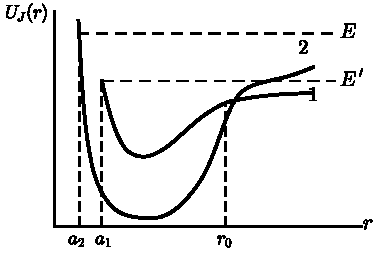
\includegraphics[width=7cm]{fig30.pdf}\\[0.3em]{\small 图 30}\end{minipage}\par\nopagebreak

另一方面，如果总能量 $E$ 位于这两个态的离解极限之上（图~30 中第一条水平虚线），从一态到另一态的跃迁相当于所谓第二类碰撞.例如 $1\to2$ 的跃迁意味着两个原子的碰撞，其结果是使两个原子处于激发态，并以减少了的动能分开（当 $r\to\infty$ 时，曲线1在曲线2的下面，$U_2(\infty)-U_1(\infty)$ 之值就是原子的激发能量）.

由于原子核的质量很大，它们的运动是准经典的.因此所考虑的跃迁概率问题属于§52中讨论过的那一类.根据该节中的一般考虑可以知道，跃迁概率主要由经典跃迁点\footnote{或者是势能变成无穷大的 $r=0$ 点.}确定.由于双原子系统（分子）的总能量在跃迁中守恒，“经典可能”的条件是两个有效势能相等：$U_{J1}(r)=U_{J2}(r)$.又由于分子的总角动量守恒，两态的离心能相同，因此这个条件意味着势能相等：
\begin{equation}
  U_1(r)=U_2(r),
\end{equation}
不再含有角动量.

如果(90.1)式在经典允许区（$E>U_{J1}$，$U_{J2}$ 的区域）内无实根，根据§52，跃迁概率是一个指数式的小量\footnote{如果参与跃迁的分子谱项可由两对不同的原子态来实现（见 §85 末），亦即势能曲线在远距离处可以分裂成为两支时，就会出现一种特殊情况.此时的跃迁概率相当大.一个例子见 А.~И.~Воронин, Е.~Е.~Никитин, Оптика и спектр. 1968. Т.~25. С.~803.}.仅当势能曲线相交于经典允许区时（如图~30 所示），跃迁概率才是显著的.此时(52.1)式中的指数幂等于零（该式也就不再适用），跃迁概率将由下面导出的非指数表式确定.这时条件(90.1)可作如下解释.如果势能（和总能）相同，两者的动量也就相同.条件(90.1)也可写成下列形式
\begin{equation}
  r_1=r_2,\qquad p_1=p_2,
\end{equation}
$p$ 是原子核相对径向运动的动量，下标1和2代表两个电子态.我们就可以这样说，跃迁发生时刻两个原子核的距离及其相对动量都保持不变（这称为弗兰克–康登原理）.从物理上讲，这是由于电子速度远大于核速度，在“电子跃迁期间”两个原子核的位置或速度不会有显著的改变.

不难确立所考虑跃迁的选择定则.首先，我们有两个明显的精确定则.总角动量 $J$ 以及谱项的符号（正或负；见§86）在跃迁中不能改变，这是因为总角动量的守恒以及坐标系反演下波函数行为的不变是任意（封闭的）多粒子系统的精确定律.

其次，宇称相异态之间的禁戒跃迁定则（由相同原子组成的分子）也是近乎精确的.态的宇称可以由核自旋和谱项符号唯一地确定.谱项符号的守恒是一个精确的定律，而核自旋是近乎守恒的，因为它和电子的作用非常弱.

要求势能曲线必须要有一个交点，这就意味着两个谱项必须具有不同的对称性（见§79）.我们来考虑微扰论一级近似下实现的跃迁（只能在高次近似下实现的跃迁，它的概率比较小）.首先要注意的是，哈密顿量中导致此跃迁的项正好就是引起能级的 $\Lambda$ 双线的项.这些项中首先有自旋–轨道作用项.它们是两个轴矢量的乘积，一个具有自旋性质（即由电子自旋算符组成），另一个具有坐标性质.但要强调指出，这两个矢量并不是简单地等于 $\hat{\boldsymbol{S}}$ 和 $\hat{\boldsymbol{L}}$ 矢量.它们对于 $S$ 和 $\Lambda$ 改变 $0,\pm1$ 的跃迁具有非零的矩阵元，其中 $\Delta S$ 和 $\Delta\Lambda$ 都等于零（同时 $\Lambda\neq0$）的情形应该除去，否则谱项的对称性将在跃迁中保持不变.两个 $\Sigma$ 谱项间的跃迁只有当一个为 $\Sigma^+$ 另一个为 $\Sigma^-$ 时才是可能的，因为一个轴矢量只对 $\Sigma^+$ 和 $\Sigma^-$ 之间的跃迁才有非零矩阵元（见§87）.

哈密顿量中对应于分子转动与轨道角动量相互作用之项是与 $\hat{\boldsymbol{J}}\cdot\hat{\boldsymbol{L}}$ 成正比的，它的矩阵元对于 $\Delta\Lambda=\pm1$ 而自旋不变的跃迁不等于零（只有矢量的 $\zeta$ 分量 $L_\zeta$ 具有 $\Delta\Lambda=0$ 的矩阵元，但是 $L_\zeta$ 对于电子态是对角的）.

除了以上考虑过的那些项以外，还有来自核动能算符（对核坐标微商的算符）的微扰，这个算符不但作用于核波函数上而且作用于以 $r$ 为参量的电子波函数上.哈密顿量中的这个相应项与未微扰哈密顿量具有同样的对称性.因此它只能导致对称性相同的电子谱项间的跃迁，由于这两个谱项并不相交，它的跃迁概率小得可以忽略.

现在来进行跃迁概率的具体计算.为确定起见，我们考虑第二类碰撞.根据一般公式(43.1)，所求的概率由下式确定：
\begin{equation}
  w=\frac{2\pi}{\hbar}\left|\int\chi_{N2}^*V(r)\chi_{N1}\,\mathrm{d}r\right|^2,
\end{equation}
其中的 $\chi_N=r\psi_N$（$\psi_N$ 为原子核径向运动波函数），$V(r)$ 是微扰能量；我们已把(43.1)式中的 $\nu_f$ 取作能量 $E$ 并且对它进行了积分.末态波函数 $\chi_{N2}$ 应按能量的 $\delta$ 函数归一化.经过这样的归一化后，(47.5)中的准经典函数具有下列形式：
\begin{equation}
  \chi_{N2}=\sqrt{\frac{2}{\pi\hbar v_2}}\,
  \cos\left(\frac{1}{\hbar}\int_{a_2}^r p_2\,\mathrm{d}r-\frac{\pi}{4}\right).
\end{equation}
归一化因子已按§21末的规则确定.初态波函数可以写成下列形式：
\begin{equation}
  \chi_{N1}=\frac{2}{\sqrt{v_1}}\,
  \cos\left(\frac{1}{\hbar}\int_{a_1}^r p_1\,\mathrm{d}r-\frac{\pi}{4}\right),
\end{equation}
它是这样归一化的，使得(90.5)式的驻波分解成两个行波后每个行波的流密度都等于1；$v_1$ 和 $v_2$ 是原子核相对径向运动的速度.当把这些函数代入(90.3)式后，即得量纲为1的跃迁概率 $w$.它可以看作原子核两次通过 $r=r_0$ 点的跃迁概率（$r_0$ 为能级的交点）.要记住，(90.5)的波函数在某种意义下相当于两次通过该点，因为它同时含有入射行波和反射行波.

由函数(90.4)和(90.5)所构成的 $V(r)$ 的矩阵元中，被积函数内含有余弦函数的乘积，这个乘积可以化成宗量为原来宗量之和及差的两个余弦函数之和.在谱项交点 $r=r_0$ 附近积分时，只有第二个余弦函数是重要的，故得
\begin{equation*}
  w=\frac{4}{\hbar^2}\left|\int\cos\left(\frac{1}{\hbar}\int_{a_1}^r p_1\,\mathrm{d}r
  -\frac{1}{\hbar}\int_{a_2}^r p_2\,\mathrm{d}r\right)
  \frac{V(r)\,\mathrm{d}r}{\sqrt{v_1v_2}}\right|^2,
\end{equation*}
离开交点时积分很快地收敛，因此可把余弦函数的宗量展为 $\xi=r-r_0$ 的幂级数并对 $\xi$ 从 $-\infty$ 到 $+\infty$ 积分（余弦函数前的缓变因子此时可用 $r=r_0$ 处的值来代替）.考虑到交点处 $p_1=p_2$，即得：
\begin{equation*}
  \int_{a_1}^r p_1\,\mathrm{d}r-\int_{a_2}^r p_2\,\mathrm{d}r
  \approx S_0+\frac{1}{2}\left(\frac{\mathrm{d}p_1}{\mathrm{d}r_0}
  -\frac{\mathrm{d}p_2}{\mathrm{d}r_0}\right)\xi^2,
\end{equation*}
其中的 $S_0$ 等于 $r=r_0$ 点处这两个积分值之差.动量的微商可通过力 $F=-\mathrm{d}U/\mathrm{d}r$ 表达出来.对等式
$\dfrac{p_1^2}{2\mu}+U_1=\dfrac{p_2^2}{2\mu}+U_2$（$\mu$ 为原子核折合质量）取微商后可得
\begin{equation*}
  v_1\frac{\mathrm{d}p_1}{\mathrm{d}r}-v_2\frac{\mathrm{d}p_2}{\mathrm{d}r}=F_1-F_2,
\end{equation*}
因此
\begin{equation*}
  \int_{a_1}^r p_1\,\mathrm{d}r-\int_{a_2}^r p_2\,\mathrm{d}r
  \cong S_0+\frac{F_1-F_2}{2v}\,\xi^2,
\end{equation*}
$v$ 为 $v_1$ 和 $v_2$ 在交点处的公共值.利用以下的熟知公式进行积分：
\begin{equation*}
  \int_{-\infty}^{+\infty}\cos(\alpha+\beta\xi^2)\,\mathrm{d}\xi
  =\sqrt{\frac{\pi}{\beta}}\cos\left(\alpha+\frac{\pi}{4}\right),
\end{equation*}
结果得
\begin{equation}
  w=\frac{8\pi V^2}{\hbar v|F_2-F_1|}
  \cos^2\left(\frac{S_0}{\hbar}+\frac{\pi}{4}\right).
\end{equation}
$S_0/\hbar$ 是一个很大的量并随能量 $E$ 很快地变化.因此即使对一段不大的能量间隔加以平均后，余弦的平方就可用它的平均值来代替.结果得下列公式：
\begin{equation}
  w=\frac{4\pi V^2}{\hbar v|F_2-F_1|}
\end{equation}
（Л.~Д.~Ландау, 1932）.式右的所有各量均取势能曲线交点处的值.

应用于预离解时，我们感兴趣的是分子在单位时间内的离解概率.振动着的原子核在单位时间内有 $2\times\dfrac{\omega}{2\pi}$ 次通过 $r=r_0$ 点.因此所求的预离解概率等于 $w$（通过两次的概率）乘以 $\omega/2\pi$，即等于
\begin{equation}
  \frac{2V^2\omega}{\hbar v|F_2-F_1|}.
\end{equation}
对于所作的这些计算应作以下说明.谈到谱项的相交时，我们所指的谱项是指分子中电子运动的“未微扰”哈密顿量 $\hat{H}_0$ 的本征值，并没有把导致跃迁的 $\hat{V}$ 项计算在内.如果在哈密顿量中包括了 $\hat{V}$ 项，谱项就不可能相交，势能曲线要略为分开，如图~31 所示.这是在§79中我们从略为不同的观点得到的结论.

\par\nopagebreak\noindent\begin{minipage}{\linewidth}\centering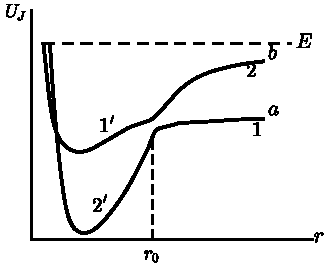
\includegraphics[width=6.5cm]{fig31.pdf}\\[0.3em]{\small 图 31}\end{minipage}\par\nopagebreak

设 $U_{J1}(r)$ 和 $U_{J2}(r)$ 为算符 $\hat{H}_0$ 的两个本征值（其中的 $r$ 看作参量）.在 $U_{J1}(r)$ 和 $U_{J2}(r)$ 曲线交点 $r_0$ 的邻域内，我们必须用§79中所示的方法去求 $\hat{H}_0+\hat{V}$ 算符的本征值 $U(r)$，结果得
\begin{equation*}
  U_{b,a}(r)=\frac{1}{2}(U_{J1}+U_{J2}+V_{11}+V_{22})\ \pm
  \sqrt{\frac{1}{4}(U_{J1}-U_{J2}+V_{11}-V_{22})^2+V_{12}^2},
\end{equation*}
式中各量都是 $r$ 的函数，$U_b(r)$ 函数（上式根号前取正号）相当于图~31 中上面一条连续曲线（$1'-2$），$U_a(r)$ 相当于下面一条曲线（$2'-1$）.$V_{11}$ 和 $V_{22}$ 矩阵元可以分别归入 $U_{J1}$ 和 $U_{J2}$ 函数的定义中；$V_{12}$ 可简记为 $V(r)$，上式变成
\begin{equation}
  U_{b,a}(r)=\frac{1}{2}(U_{J1}+U_{J2})
  \pm\frac{1}{2}\sqrt{(U_{J1}-U_{J2})^2+4V^2},
\end{equation}
能级间距为
\begin{equation}
  \Delta U=\sqrt{(U_{J1}-U_{J2})^2+4V^2}.
\end{equation}
由此可见，如果两态间有跃迁（$V\neq0$），能级的相交就不存在.曲线间的最短距离位于 $r=r_0$ 处，该处的 $U_{J1}=U_{J2}$，故得
\begin{equation}
  (\Delta U)_{\min}=2|V(r_0)|
\end{equation}
在这点附近，我们把差值 $U_{J1}-U_{J2}$ 展为 $\xi=r-r_0$ 的幂级数，令
\begin{equation*}
  U_{J1}-U_{J2}=U_1-U_2\approx\xi(F_2-F_1),
\end{equation*}
其中 $F=-(\mathrm{d}V/\mathrm{d}r)_{r_0}$，则
\begin{equation}
  \Delta U=\sqrt{(F_2-F_1)^2\xi^2+4V^2(r_0)}.
\end{equation}
(90.11)和(90.12)式是在只考虑两个态的情况下导出的，这两式的成立要求 $(\Delta U)_{\min}$ 必须小于其它谱项的间距.(90.7)式作为跃迁概率必须满足后面更为严格的条件(90.19).如果后一条件并不满足，仍容许只考虑两个态，但不能用通常微扰论计算跃迁概率，这种情形下需要更一般的处理.

如果我们只考虑交点的邻区并把核运动作准经典处理，那么系统哈密顿量中的核速度算符可用常数 $v$ 代替，坐标 $r$ 可以作为时间的函数满足经典方程 $\mathrm{d}r/\mathrm{d}t=v$，亦即 $\xi=r-r_0=vt$.计算跃迁概率的问题就化成求解电子波函数所满足的波动方程，它的哈密顿量显含时间 $t$：
\begin{equation}
  \mathrm{i}\hbar\frac{\partial}{\partial t}\varPsi
  =\bigl[\hat{H}_0(t)+\hat{V}(t)\bigr]\varPsi.
\end{equation}
令 $\psi_a$ 和 $\psi_b$ 为对应于曲线 $a$ 和 $b$ 的电子态的波函数.它们是下式之解
\begin{equation*}
  (\hat{H}_0+\hat{V})\psi_{a,b}=U_{a,b}(t)\psi_{a,b},
\end{equation*}
式中 $t$ 是一个参量.把(90.13)之解取作下列形式：
\begin{equation}
  \varPsi=a(t)\psi_a+b(t)\psi_b.
\end{equation}
如果方程按 $t\to-\infty$ 时 $a=1$，$b=0$ 的边界条件求解，则 $|b(\infty)|^2$ 给出分子进入 $\psi_b$ 态的概率，代表原子核通过 $r=r_0$ 点时从曲线 $a$ 到曲线 $b$ 的跃迁.同理，$|a(\infty)|^2=1-|b(\infty)|^2$ 为分子仍留于曲线 $a$ 的概率.两次通过 $r_0$ 点（两核先接近再分开）的过程中从曲线 $a$ 到曲线 $b$ 的跃迁可以有两种方式：$a\to b\to b$（接近时有 $1\to1'$ 跃迁，分开时分子留在 $1'2$ 曲线上），或者 $a\to a\to b$（接近时 $1\to2'$，分开时 $2'\to2$），因此所求的跃迁概率为
\begin{equation}
  w=2|b(\infty)|^2\bigl[1-|b(\infty)|^2\bigr],
\end{equation}
式中引用了这样的事实，即通过 $r=r_0$ 点的跃迁概率当然和运动方向无关.

$b(\infty)$ 的值可以用§53中描述的方法求出，不必直接应用(90.13)式\footnote{§53 中，我们假定了过程是完全绝热的，因此求得的概率是指数式小量.但在目前情形下，当两核就在 $r_0$ 点的邻域内，它们的速度 $v$ 如果不足够小的话，这个条件可能被破坏.可是，根据 §52 和 §53 中的分析可以清楚地看到，对该法本身的可用性而言，只有下列两点是重要的，即当 $|t|$ 大时的绝热性以及只限于两个能级.}.为此，我们注意到 $U_a(t)$ 和 $U_b(t)$ 曲线相交于下列虚点：
\begin{equation}
  t_0^{(\pm)}=\pm\mathrm{i}\,\frac{2|V|}{|F_2-F_1|v}\equiv\pm\mathrm{i}\tau_0,
\end{equation}
对很大的负 $t$ 值，(90.14)中的系数 $a(t)$ 具有下列“对时间为准经典”的形式：
\begin{equation*}
  a(t)=\exp\left\{-\frac{1}{\hbar}\int_{-\infty}^t U_a(t)\,\mathrm{d}t\right\}.
\end{equation*}
在 $t$ 复平面上，我们从左实轴出发沿着“准经典”条件总能满足的回线到达右实轴，由于 $U_a<U_b$，所取回线一定在上半平面内绕过 $t_0^{(+)}$ 点（参考§53）.$a(t)$ 函数就变成 $b(t)$，而
\begin{equation*}
\begin{aligned}
  |b(\infty)|^2&=\exp\bigg\{\frac{2}{\hbar}\mathrm{Im}\bigg[\int_{t_1}^{\mathrm{i}\tau_0}U_a(t)\,\mathrm{d}t
  +\int_{\mathrm{i}\tau_0}^{t_1}U_b(t)\,\mathrm{d}t\bigg]\bigg\}=\\
  &=\exp\bigg\{-\frac{2}{\hbar}\mathrm{Im}\int_{t_1}^{\mathrm{i}\tau_0}\Delta U\,\mathrm{d}t\bigg\},
\end{aligned}
\end{equation*}
$t_1$ 可取实轴上任一点，例如 $t_1=0$.按(90.12)，我们有
\begin{equation}
  \Delta U=\sqrt{(F_2-F_1)^2v^2t^2+4V^2},
\end{equation}
作替换 $t=\mathrm{i}\tau$ 后所求积分变成
\begin{equation*}
  \mathrm{i}\int_0^{\tau_0}\sqrt{4V^2-(F_2-F_1)^2v^2\tau^2}\,\mathrm{d}\tau
  =\mathrm{i}\,\frac{\pi V^2}{v|F_2-F_1|}.
\end{equation*}
由此我们得到跃迁概率的下列最终表式：
\begin{equation}
  w=2\exp\left(-\frac{2\pi V^2}{\hbar v|F_2-F_1|}\right)
  \left[1-\exp\left(-\frac{2\pi V^2}{\hbar v|F_2-F_1|}\right)\right]
\end{equation}
（C.~Zener, 1932）.我们可以看出，在两种极限情形下跃迁概率都变得很小.当 $V^2\gg\hbar v|F_2-F_1|$ 时，它是一个指数式小量（绝热情形）；当
\begin{equation}
  V^2\ll\hbar v|F_2-F_1|,
\end{equation}
时(90.18)变成(90.7)式.由(90.17)式知，$\tau\sim|V|/(|F_2-F_1|v)$ 是原子核通过交点的“通过时间”，相应的频率为 $\omega_\tau\sim1/\tau$.以上两种极限情形能否达到，由 $\hbar\omega_\tau$ 和该问题中的特征能量 $|V|$ 之间的关系来确定.

最后，我们来考虑一个类似于预离解的现象，称为双原子分子光谱中的微扰.如果有两个离散的分子能级 $E_1$ 和 $E_2$，对应于两个相交的电子谱项，彼此靠得很近，那么这两个电子态之间的跃迁可能性会引起能级的位移.根据微扰论的一般公式(79.4)，位移能级的表式为
\begin{equation}
  \frac{E_1+E_2}{2}\pm
  \sqrt{\left(\frac{E_1-E_2}{2}\right)^2+|V_{12N}|^2},
\end{equation}
式中的 $V_{12N}$ 是分子态1和2之间跃迁的微扰矩阵元；矩阵元 $V_{11N}$ 和 $V_{22N}$ 显然已包括在 $E_1$ 和 $E_2$ 内.由上式可知，这两个能级背向移动而分开（高能级上升另一能级下降）.差值 $|E_1-E_2|$ 愈小位移量则愈大.

矩阵元 $V_{12N}$ 的计算方法是和确定第二类碰撞的概率所用的方法相同.唯一的差别是，现在的波函数 $\chi_{N1}$ 和 $\chi_{N2}$ 都属于离散谱，因此都必须归一化为1.根据(48.3)式我们有
\begin{equation*}
  \chi_{N1}=\sqrt{\frac{2\omega_1}{\pi v_1}}\,
  \cos\left(\frac{1}{\hbar}\int_{a_1}^r p_1\,\mathrm{d}r-\frac{\pi}{4}\right),
\end{equation*}
对 $\chi_{N2}$ 有类似的式子.与(90.3)到(90.5)诸式比较后可知，目前考虑的矩阵元 $V_{12N}$ 与两次通过交点时的那个跃迁概率 $w$ 之间具有下列关系：
\begin{equation}
  |V_{12N}|^2=w\,\frac{\hbar\omega_1}{2\pi}\,\frac{\hbar\omega_2}{2\pi}.
\end{equation}

\begin{xiti}

\noindent{\heiti 习题1}\quad 试求第二类碰撞的总截面并把它表为相碰原子动能 $E$ 的函数，跃迁是由自旋轨道作用引起的（朗道，1932）.

解：考虑到核运动的准经典性，可引入碰撞参量 $\rho$ 的概念（$\rho$ 即不考虑原子核的相互作用时入射原子核的偏射距离），并把有效截面 $\mathrm{d}\sigma$ 定义为“靶面积” $2\pi\rho\,\mathrm{d}\rho$ 与每次碰撞时的跃迁概率 $w(\rho)$ 的乘积（参考《力学》，§18）.对 $\rho$ 积分后即得总截面 $\sigma$.

对于自旋–轨道作用，矩阵元 $V(r)$ 与相碰原子的角动量 $M$ 无关.我们把曲线交点 $r=r_0$ 处的速度 $v$ 写成下列形式：
\begin{equation*}
  v=\sqrt{\frac{2}{\mu}\left(E-U-\frac{M^2}{2\mu r_0^2}\right)}
  =\sqrt{\frac{2}{\mu}\left(E-U-\frac{\rho^2E}{r_0^2}\right)},
\end{equation*}
其中的 $U$ 是 $U_1$ 和 $U_2$ 在交点处的公共值，$\mu$ 是两原子的折合质量，角动量 $M=\mu\rho v_\infty$，$v_\infty$ 是两原子相距无穷远时的相对速度.选择能量的零点，使得初态中原子的相互作用能量在无穷远处等于零，此时有 $E=\mu v_\infty^2/2$.代入(90.7)式得：
\begin{equation*}
  \mathrm{d}\sigma=2\pi\rho\,\mathrm{d}\rho\,w
  =\frac{8\pi^2V^2}{\hbar|F_2-F_1|}
  \frac{\rho\,\mathrm{d}\rho}{\sqrt{\dfrac{2}{\mu}\left(E-U-\dfrac{\rho^2E}{r_0^2}\right)}}.
\end{equation*}
对 $\mathrm{d}\rho$ 的积分应从零开始到速度 $v$ 等于零时的 $\rho$ 值为止.结果得：
\begin{equation*}
  \sigma=\frac{4\sqrt{2\mu}\,\pi^2V^2r_0^2}{\hbar|F_2-F_1|}
  \frac{\sqrt{E-U}}{E}.
\end{equation*}

\noindent{\heiti 习题2}\quad 同上题，但跃迁是由分子转动与轨道角动量间的相互作用引起的（朗道，1932）.

解：矩阵元 $V$ 呈 $V(r)=MD/\mu r^2$ 的形式，其中的 $D(r)$ 是电子轨道角动量的矩阵元.应用和题1相同的方法，得：
\begin{equation*}
  \sigma=\frac{16\sqrt{2}\,\pi^2D^2}{3\hbar\sqrt{\mu}\,|F_2-F_1|}
  \frac{(E-U)^{3/2}}{E}.
\end{equation*}

\noindent{\heiti 习题3}\quad 当能量 $E$ 接近于交点处的势能值 $U_J$ 时，求跃迁概率.

解：当 $E-U_J$ 值很小时，(90.7)式不能适用，由于交点附近的核速度 $v$ 不能看作常数，因此不能像推导(90.7)式那样把它拿出积分号外.

交点附近的 $U_{J1}$，$U_{J2}$ 曲线可改成两条直线：
\begin{equation*}
  U_{J1}=U_J-F_{J1}\xi,\qquad
  U_{J2}=U_J-F_{J2}\xi,\qquad
  \xi=r-r_0.
\end{equation*}
这个区域内的波函数 $\chi_{N1}$ 和 $\chi_{N2}$ 就是均匀场中一维运动的波函数（§24）.为计算方便，我们采用动量表象中的波函数.按能量的 $\delta$ 函数归一化后的波函数具有下列形式（见§24例题）：
\begin{equation*}
  a_2=\frac{1}{\sqrt{2\pi\hbar|F_{J2}|}}\,
  \exp\left\{\frac{\mathrm{i}}{\hbar F_{J2}}
  \left[(E-U_J)p-\frac{p^3}{6\mu}\right]\right\},
\end{equation*}
乘以 $\sqrt{2\pi\hbar}$ 后，可得按入射波和反射波的单位流密度归一化的波函数：
\begin{equation*}
  a_1=\frac{1}{\sqrt{|F_{J1}|}}\,
  \exp\left\{\frac{\mathrm{i}}{\hbar F_{J1}}
  \left[(E-U_J)p-\frac{p^3}{6\mu}\right]\right\}.
\end{equation*}
积分时，微扰能（矩阵元）$V$ 又有可能拿到积分号外，并用它在交点处的值来代替：
\begin{equation*}
  w=\frac{2\pi}{\hbar}\left|V\int_{-\infty}^{+\infty}a_1a_2^*\,\mathrm{d}p\right|^2,
\end{equation*}
结果得：
\begin{equation*}
  w=\frac{4\pi V^2(2\mu)^{2/3}}{\hbar^{4/3}(F_{J1}F_{J2})^{1/3}(F_{J2}-F_{J1})^{2/3}}\,
  \varPhi^2\left[-(E-U_J)\left(\frac{2\mu}{\hbar^2}\right)^{1/3}
  \left(\frac{1}{F_{J2}}-\frac{1}{F_{J1}}\right)^{2/3}\right],
\end{equation*}
式中的 $\varPhi(\xi)$ 是艾里函数（见数学附录§b）.当 $E-U_J$ 很大时上式变成(90.7)式.

\noindent{\heiti 习题4}\quad 试求一个氢原子和一个氢离子（质子）远而慢的碰撞（即相对速度 $v\ll1$）中的电荷交换概率（О.~Б.~Фирсов, 1951）.\footnote{本题用原子单位}

解：我们把 $\mathrm{H}+\mathrm{H}^+$ 系统看作一个电离氢分子（见§81题），电荷交换是由于电子从核1处的 $\psi_1$ 态过渡到核2附近的 $\psi_2$ 态.即便原子核是静止的，这些态都不是定态.定态为
\begin{equation*}
  \psi_{g,u}=\frac{1}{\sqrt{2}}(\psi_1\pm\psi_2),
\end{equation*}
它们的能量 $U_{g,u}(R)$ 是核距离 $R$ 的函数.当核作给定的慢运动（看作经典运动）时，这些能量是时间的缓变函数，波函数对时间的依赖关系由“对时间的准经典”因子给出（对照§53）：
\begin{equation*}
  \exp\left(-\mathrm{i}\int U_{g,u}(t)\,\mathrm{d}t\right).
\end{equation*}
$t\to-\infty$ 时等于 $\psi_1$ 的那个叠加态为
\begin{equation*}
  \varPsi=\frac{1}{\sqrt{2}}\bigg[\psi_g\exp\left(-\mathrm{i}\int_{-\infty}^t U_g\,\mathrm{d}t\right)
  +\psi_u\exp\left(-\mathrm{i}\int_{-\infty}^t U_u\,\mathrm{d}t\right)\bigg],
\end{equation*}
$t\to\infty$ 时，上式呈 $c_1\psi_1+c_2\psi_2$ 线性组合形式，电荷交换概率为 $w=|c_2|^2$.简单计算后得
\begin{equation*}
  w=\sin^2\eta,\qquad
  \eta=\frac{1}{2}\int_{-\infty}^{\infty}(U_u-U_g)\,\mathrm{d}t.
\end{equation*}
在碰撞参量 $\rho$ 很大（同时速度 $v$ 够慢）的碰撞中，核运动可以假定在 $R=\sqrt{\rho^2+v^2t^2}$ 的一条直线上，$R\gg1$ 时的差值 $U_u-U_g$ 已由§81例题中(4)式给出.此时
\begin{equation*}
  \eta=\frac{4}{v}\int_\rho^\infty
  \frac{R^2\mathrm{e}^{-R-1}}{\sqrt{R^2-\rho^2}}\,\mathrm{d}R,
\end{equation*}
$\rho\gg1$ 时，这个积分中 $R$ 值的重要区域位于积分下限附近.令 $R=\rho(1+x)$，我们得
\begin{equation*}
  \eta=\frac{2\sqrt{2}}{e\,v}\,\rho^2\mathrm{e}^{-\rho}
  \int_0^\infty\frac{\mathrm{e}^{-\rho x}}{\sqrt{x}}\,\mathrm{d}x
  =\frac{2\sqrt{2\pi}}{e\,v}\,\rho^{3/2}\mathrm{e}^{-\rho}.
\end{equation*}

\end{xiti}
